\documentclass[11pt]{article}
\usepackage[margin=1in]{geometry}
\usepackage[T1]{fontenc}
\usepackage[utf8]{inputenc}
\usepackage{lmodern,microtype}
\usepackage{graphicx,booktabs,longtable,array,multirow}
\usepackage{amsmath,amssymb}
\usepackage[hidelinks]{hyperref}
\usepackage{caption}
\captionsetup{font=small,labelfont=bf}
\usepackage{natbib}
\setlength{\parskip}{2pt}

\title{Institutional Positioning from 13F Filings:\\
Point-in-Time Data Engineering, a Signal Taxonomy,\\
and What Survived a Pre-Registered Research Funnel}
\author{Lucas Silva}
\date{August 2026}

\begin{document}
\maketitle

\begin{abstract}
\noindent We build a point-in-time research system for SEC 13F
institutional holdings --- bitemporal storage keyed on filing
acceptance, amendment semantics from cover pages, a
CUSIP$\to$name$\to$current-ticker crosswalk with human-in-the-loop
resolution --- and run a pre-registered research funnel over six
classes of positioning signals. Two objects survive. The first,
\emph{New-Conviction Breadth} (NCB): the cross-section of filers
opening or materially growing top-decile-of-book positions,
residualized on size and liquidity, earns $+1.9\%$ per quarter in
quintile spreads ($t=+3.4$, Sharpe $\approx 1.0$), replicates eight
times across two universes and four implementations, and its full
$36$-point hyperparameter surface is positive out-of-sample. The
second, \emph{Forced-Sale Supply} (FSS): managers whose implied flow
falls below $-10\%$ sell $34.5\%$ of held shares the following quarter
against $23.1\%$ for healthy managers ($t\approx+10$ at every
threshold), and the resulting supply basket prices as a
regime-dependent short. Around these survivors we document, with the
same protocol, why almost everything else fails: fifteen crowding
formulations, nine smart-money designs, five pre-registered
interaction effects, and daily anticipation of institutional stress
--- one instance of which we retract explicitly after a data-coverage
audit, and the audit itself (46\% of book value initially unmapped by
name matching) is presented as a core result. A Fama--MacBeth
combiner over ten characteristics is the production model (OOS Sharpe
$0.86$); IPCA and gradient-boosted alternatives are evaluated and
held at candidate status by the funnel's own promotion rules. Two
empirical regularities organize every outcome: ownership
\emph{states} carry no directional information at any clock, and
alpha lives only where the observed action was \emph{costly}
(conviction displacement) or \emph{forced} (redemption-driven
liquidation).
\end{abstract}

\tableofcontents
\newpage

\section{Introduction}
\label{sec:intro}

Quarterly 13F filings are the most complete public record of
institutional equity positioning, and the most heavily mined. The
literature's box score is mixed by construction: the filings are
stale (up to 45 days), long-only, and quarterly, so most of what they
reveal is already in prices. Our starting premise is therefore not
``institutions know something,'' but a narrower mechanical claim:
\emph{the filings occasionally reveal actions that were either costly
to take or impossible to avoid}, and only those actions should carry
a premium. A manager displacing an existing top-decile position to
make room for a new name has paid a real price for that opinion; a
manager liquidating a third of a book under redemptions is not
expressing an opinion at all. Everything in this report is organized
around whether a signal isolates one of those two situations.

The work divides into three parts. The first
(Sections~\ref{sec:data}--\ref{sec:universe}) is data engineering,
and we give it the space usually reserved for results because in this
dataset the engineering \emph{is} the result: a bitemporal
point-in-time store keyed on filing acceptance timestamps; amendment
semantics read from cover pages rather than guessed; per-filing value
scale detection; a CUSIP$\to$issuer-name$\to$current-ticker crosswalk
with human resolution of edge cases; and a value-weighted coverage
audit that late in the project found 46.4\% of book value unmapped
--- EDGAR's name abbreviations defeat exact matching precisely on the
mega-caps --- forcing a fix and a 24-run re-verification campaign in
which one previously reported result was retracted
(Section~\ref{sec:campaign}). We report the retraction with its
mechanism because the episode is the strongest evidence we can offer
that the rest of the numbers mean something.

The second part (Sections~\ref{sec:taxonomy}--\ref{sec:fss}) is a
taxonomy: six classes of positioning signals, seventeen catalogue
constructions evaluated under one fixed protocol, five pre-registered
interaction effects, and the two survivors. New-Conviction Breadth
(NCB) counts, per stock, the fraction of filers that opened or grew
($\ge 25\%$, split-adjusted) a position sitting in the top decile of
their own book, residualized on size and dollar liquidity because a
formal placebo (``dart-throwing value-weighted managers'') shows the
raw count is mechanically correlated with both. Forced-Sale Supply
(FSS) converts a validated manager-level flow instrument into a
stock-level supply measure. For each we present the economic
mechanism first, the returns second, and the hyperparameter surface
third --- every parameter in this report is either justified by a
measurement or explicitly labeled a convention.

The third part (Sections~\ref{sec:models}--\ref{sec:limitations})
assembles the pieces into production objects and stress-tests the
assembly: a Fama--MacBeth expected-return combiner over ten
characteristics (the production model), an IPCA challenger under the
\citet{kps2019} instrumented-loadings framework, a gradient-boosted
ex-post exercise that rediscovers NCB and finds no nonlinear premium,
net-of-cost engine results with explicit commission and borrow
accounting, and the descriptive context --- the median large 13F
filer underperforms the S\&P~500 by $3.3\%$ per year before fees ---
that explains why imitating these books is a losing design and
harvesting their \emph{flows} is not.

Two regularities recur so often that we state them as laws and tag
every result with them. \textbf{Law 1: states have no arrow.} Levels
of ownership, breadth, crowding, concentration, or factor tilt never
predict returns in this data, at any clock, in fifteen independent
formulations; changes and constrained actions do. \textbf{Law 2:
distress is information when observed, never when predicted.}
Contemporaneous forced selling is measurable with $t\approx+10$;
every attempt to anticipate it --- daily synthetic stress, quarterly
flow forecasting, single-name crash cascades --- fails its mechanism
gate or dies on the full panel.

\section{Data engineering: from EDGAR to a point-in-time store}
\label{sec:data}

\subsection{Ingestion and storage}

Two ingestion paths run in parallel by design. The SEC DERA
structured datasets ($\sim$53 quarterly archives) are cheap and carry
the other-manager graph, but begin in 2013Q2 and inherit the SEC's
own parsing unaudited. The raw-filing path (SGML envelopes; XML after
2013, fixed-width layouts before) covers the whole archive and is
auditable, at one HTTP request per filing. A cross-validation routine
re-parses a random sample of raw filings and compares row counts and
value totals against DERA; neither source can check itself, and
agreement below 95\% halts the pipeline. The sample begins in 2013Q2
where the two paths overlap and the structured OTHERMANAGER graph is
available --- earlier eras are parseable but single-sourced, and we
prefer a shorter sample with a second witness.

Every holding row carries two dates: the period it describes and the
timestamp at which it became public (EDGAR acceptance). The store's
only read path for research, \texttt{as\_of(period, knowledge\_date)},
materializes both the current and prior quarter at the same knowledge
date, so a quarter-over-quarter change never mixes what was known
then with what is known now. Three mechanical look-ahead channels are
closed at this layer: late filings (a filer's book enters the panel
only after its acceptance timestamp), amendments (a correction
filed in March cannot retroactively improve a January decision), and
restatement semantics.

\subsection{Amendments, value scale, identity}

Amendment handling follows the cover page, never a heuristic:
\texttt{RESTATEMENT} replaces the filer's table for the period;
\texttt{NEW HOLDINGS} is additive (typically a lapsed
confidential-treatment order); a missing declaration is treated as a
restatement, the conservative choice. Misreading an additive
amendment as a restatement silently deletes a quarter's book ---
this failure mode is pinned by a test. An amendment is a
\emph{version} of its original, and never competes with it in any
largest-book logic. Value scale (the 2022--2023 thousands-to-dollars
cutover) is detected per filing keyed on the \emph{filing} date, with
loud outlier flags for the tail of filers that ignores the rule.
Filer identity is resolved by union-find over explicit evidence
(shared filings, CIK succession); name-similarity methods only
propose, and any merge requires a manual entry in a reviewed
configuration file --- nothing in the pipeline merges on string
distance alone.

\subsection{When information actually arrives}
\label{sec:delays}

The decision clock used throughout is quarter-end $+45$ calendar
days, the statutory deadline. Table~\ref{tab:delays} and
Figure~\ref{fig:delays} justify it with the acceptance-timestamp
distribution over 254{,}630 original filings: the median filer
reports 41 days after quarter end, half of all filings arrive in the
final five days before the deadline, 89.4\% have arrived by D+45 and
98.1\% by D+60; the 99th percentile is 128 days and the maximum
observed 400. Lateness is sticky (a filer late once is late again
41\% of the time), so late books are a persistent subpopulation, not
noise. A per-name ragged-entry design --- entering each stock on the
day its holder's filing actually arrived --- adds $+0.2\%$/yr
($t\approx 0$) over the batch clock (Section~\ref{sec:tactical}): the
information is so concentrated at the deadline that waiting for it
costs nothing.

\begin{table}[t]
\centering\small
\caption{Filing-delay distribution, original 13F filings 2013--2026
($n=254{,}630$). The D+45 batch clock is justified by measurement:
89\% of books are public by the statutory deadline and the ragged
per-name alternative adds nothing (Section~\ref{sec:tactical}).}
\label{tab:delays}
\begin{tabular}{lrrrrrrr}
\toprule
 & median & p90 & p99 & max & $\le$D+40 & $\le$D+45 & $\le$D+60 \\
\midrule
delay (days) & 41 & 46 & 128 & 400 & 49.9\% & 89.4\% & 98.1\% \\
\bottomrule
\end{tabular}
\end{table}

\begin{figure}[t]
\centering
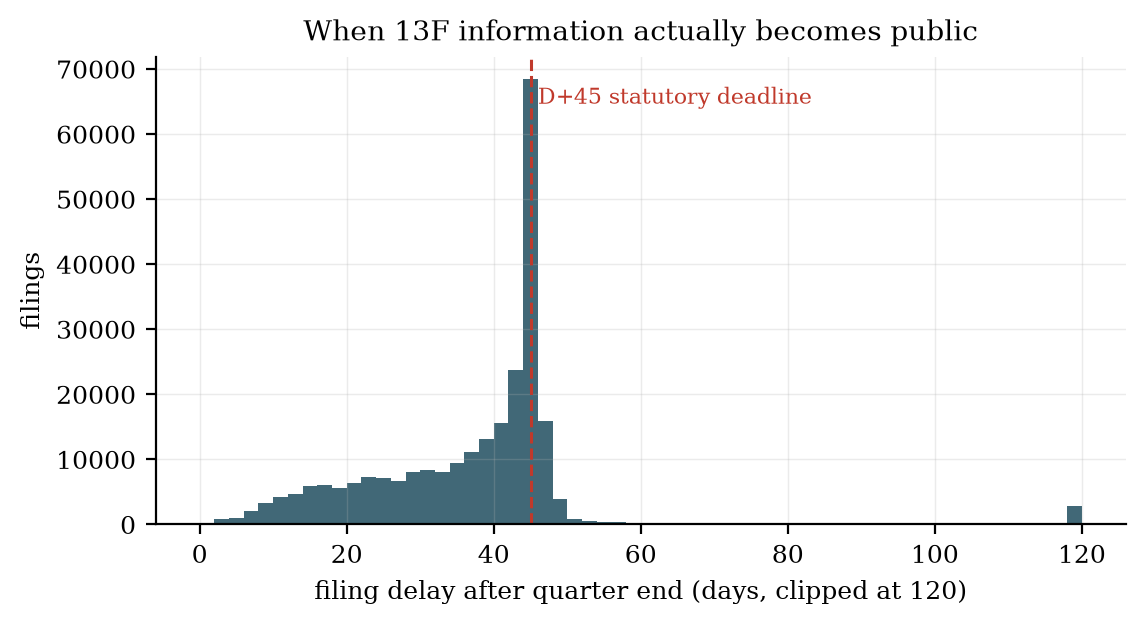
\includegraphics[width=.72\linewidth]{figs/f9_delays.png}
\caption{Acceptance-timestamp distribution. Half of all filings land
in the last five days before the statutory deadline (dashed line).}
\label{fig:delays}
\end{figure}

\subsection{The crosswalk, and the audit that mattered}
\label{sec:crosswalk}

Holdings identify securities by CUSIP; the price panel is keyed by
ticker. The map is CUSIP $\to$ issuer name (from the filings
themselves) $\to$ \emph{current} ticker by normalized-name match
against the exchange directory, ambiguous names discarded, with
manual resolution of edge cases (human in the loop). Three failure
modes were analyzed separately. Ticker renames (\texttt{FB}$\to$%
\texttt{META}) are correct by construction, because the vendor
reindexes history under the current symbol. Ticker recycling fails
\emph{closed}: history of a delisted issuer is never spliced under a
recycled symbol, so affected periods drop out at the price floor ---
exclusion, never mispricing (4.5\% of tickers flagged; inspected
cases are known spin-offs and IPOs). CUSIP reassignment by the same
issuer --- the genuine blind spot --- was measured directly: 1{,}574
events over 51 quarters, contaminating 0.22\% of position-exit flow;
exit-based signals are safe uncorrected.

Late in the project a value-weighted audit --- prompted by the simple
question ``what happens when tickers change?'' --- found that
\textbf{46.4\% of 2025Q4 book value was unmapped}. The cause was not
renames but EDGAR's name abbreviations (``LILLY ELI \& CO'',
``INTERNATIONAL BUSINESS MACHS''), which defeat exact matching
precisely on the mega-caps every value book holds. Count-weighted
coverage had looked healthy throughout; the lesson we record is that
\emph{coverage audits must be value-weighted}. The fix: the top 250
unmapped CUSIPs by value (65\% of the hole) hand-mapped and verified
individually; 61 new price histories fetched; caches stitched;
non-ETF value coverage raised from 63\% to 85.4\%, with a documented
ladder to $\sim$93\% (identifier-service tail) and $\sim$98\%
(CRSP-tier, delistings).

\subsection{The re-verification campaign and one retraction}
\label{sec:campaign}

Because coverage selection could in principle manufacture or hide
results, every material verdict was re-run on the expanded universe:
24 re-runs. The pre-registered expectation was that the hole was
quasi-random with respect to signals (EDGAR name formatting does not
predict returns), so levels could move where mega-caps matter but
verdicts should stand. Twenty-one verdicts were unchanged; two
instruments \emph{strengthened} with completer books (the flow
instrument's selling contrast from $t=+13.8$ to $t=+20.9$; synthetic
short interest's correlation with actual short interest from $0.47$
to $0.55$); NCB replicated inside its historical band and survived
two random 50\%-coverage halvings ($t=+3.45/+2.79$), the generic
proof that quasi-random coverage cannot flip verdicts.

One result flipped and is retracted: a daily overlay claiming that a
synthetically detected ``stressed'' manager's top holdings
underperform over the following five days ($t=-2.16$ on the old
universe) went to $t=+0.37$ on complete books and is dead even inside
its own sub-window. The diagnosis is an eligibility-selection
artifact: coverage filters had excluded managers holding unmapped
mega-caps, biasing the manager sample toward a stratum where the
effect appeared. The research funnel had already declined to promote
the result (net returns too thin); the audit converted ``not
promotable'' into ``false.'' We keep both the machinery (reused by
the risk monitors of Section~\ref{sec:tactical}) and the negative
finding.

\section{The manager universe: a census, not a chosen list}
\label{sec:universe}

The filer universe is the full census of 13F filers each quarter ---
2{,}793 in 2013Q2 growing to 7{,}693 by 2026Q1
(Figure~\ref{fig:universe}) --- and this is a deliberate result, not
a default. Five families of eligibility filters were tested against
the census with paired quarter-by-quarter deltas on identical stocks:
activity and concentration screens (four variants), long-horizon
``patient'' managers, top-past-performer screens, passive-manager
exclusions, and ETF purges. Every filter either hurt (activity
screens up to $t=-2.54$; patient screens $t=-2.35$ to $-3.25$) or did
nothing. The votes discarded with the managers carried information;
the electorate is not the dial that matters
(Section~\ref{sec:ncb-surface} shows the dial that does --- the
definition of the vote itself).

\begin{figure}[t]
\centering
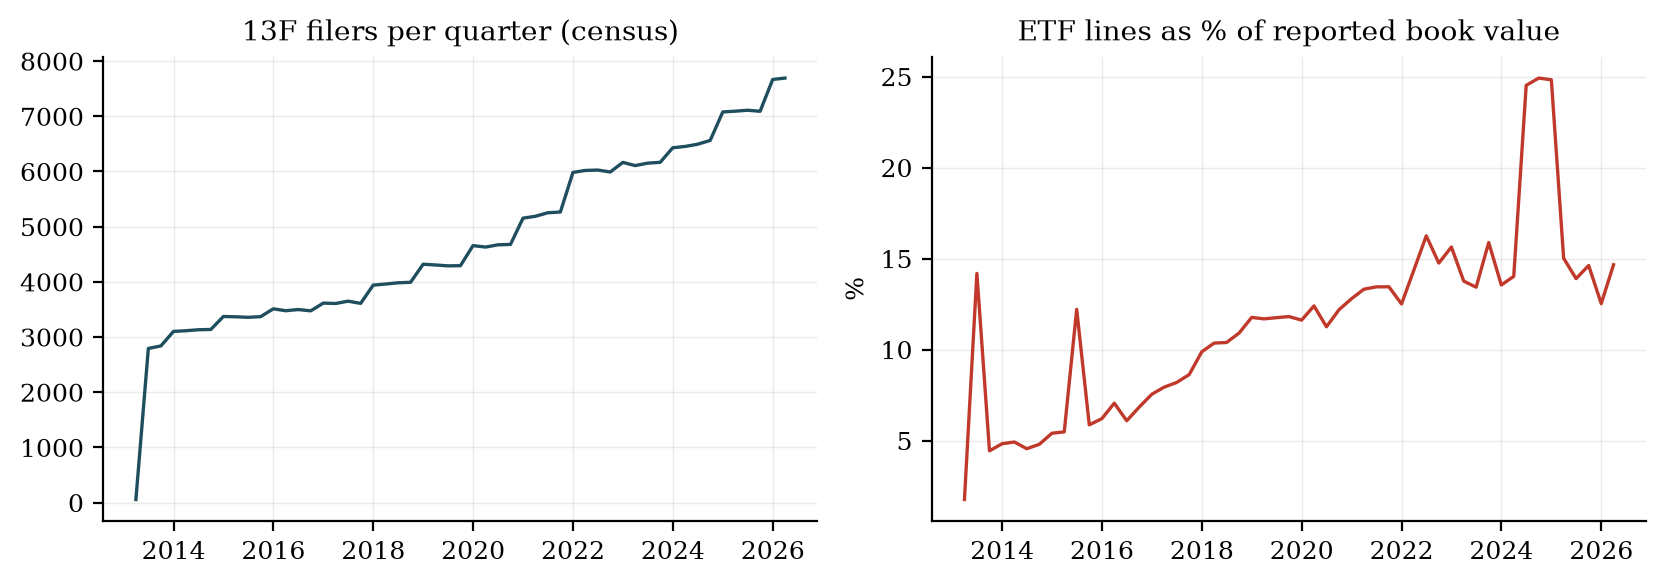
\includegraphics[width=.95\linewidth]{figs/f10_universe.png}
\caption{Left: 13F filers per quarter (census). Right: ETF lines as a
share of reported book value --- material and growing, and measured
to be innocuous for ranking signals (uniform, not differential,
contamination).}
\label{fig:universe}
\end{figure}

\paragraph{The ETF and passive-manager question.}
Because index products are 12--15\% of reported book value
(Figure~\ref{fig:universe}, right), we closed this question on three
independent fronts rather than by assumption. (i) \emph{Tradable
universe}: of 7{,}886 audited ETF instruments, one appears in the
crosswalk and none in the price panel --- ETFs were never buyable in
any backtest. (ii) \emph{Inside books}: purging ETF lines from filer
books changes the conviction threshold of $\sim$25\% of managers per
quarter and releases 17\% more conviction votes (single-stock bets
hidden behind index positions), yet the stock-level ranking is
unchanged (rank correlation $0.974$; top-100 overlap 97/100; paired
delta $+0.01\%$/quarter, $t=+0.08$): uniform contamination does not
distort a ranking signal. (iii) \emph{Passive managers as voters}:
only $\sim$10 filers per quarter have active share below 25\% --- the
giant index complexes, one third of aggregate AUM --- and they
produce $\sim$1\% of conviction votes; removing them moves the spread
by six basis points ($t=+1.19$). We summarize the asymmetry as
\emph{elephants without votes}: cutting active managers hurts,
cutting passive ones is noise, and the census stands on measured
parsimony.

\paragraph{Tradable asset universe.}
Common equities with a mapped current ticker and price
$\ge\$1$; no ADV floor at the signal-evaluation layer (the
illiquid short side is where several literature effects live), with
liquidity entering explicitly through each signal's denominator or
the engine's cost model rather than through silent universe
truncation. The production engine (Section~\ref{sec:engine}) applies
its own stricter tradability filter ($\$4$ price, $\$5$M median
dollar volume, 252 days of history).

\section{Evaluation protocol and research discipline}
\label{sec:protocol}

All signal evaluations share one protocol, fixed before any return
was examined. Decisions at quarter-end $+45$ days (justified in
Section~\ref{sec:delays}); holdings via the point-in-time store;
quintile portfolios, equal-weighted primary and value-weighted
reported; Q5$-$Q1 spreads on forward quarterly returns;
Newey--West $t$-statistics (4 lags); Spearman rank information
coefficients; a \$1 price floor; ties broken by seeded random jitter
(deterministic alphabetical tie-breaking is an artifact generator
where sorts have mass points at zero). Cumulative-return figures are
log-scale throughout.

Two statistical conventions are worth stating precisely. Forward
quarterly returns are \emph{sums of daily simple returns} --- a
log-return approximation that ignores intra-window compounding. It is
applied identically on both sides of every sort, so spreads are
quintile-neutral to the convention; reported levels are mildly
conservative for high-volatility names. Newey--West with four lags on
\emph{non-overlapping} quarterly series is deliberately conservative:
the spreads carry no mechanical overlap, so the correction can only
widen standard errors against residual autocorrelation and
volatility clustering.

\paragraph{Why equal weights as the measurement base.}
The evaluation question is cross-sectional: \emph{does the ranking
order next-quarter returns?} Under that question every name is one
observation, so the diagnostic portfolio weights names equally ---
value-weighting re-asks the question ``does it order returns among
mega-caps?'', a narrower hypothesis whose spread variance is
dominated by a handful of names (the effective $N$ collapses, and
with it the fundamental-law arithmetic $\mathrm{IR}\approx
\mathrm{IC}\sqrt{N}$ that our signals live on). EW is therefore the
\emph{measurement} convention and cap-weighting the
\emph{implementation} convention: the tradability question EW raises
(small-cap loading) is answered downstream and explicitly --- the
engine trades a filtered universe with costs
(Section~\ref{sec:engine}), and the long-only product is built on
cap weights with a tilt (Section~\ref{sec:lo}). VW variants are
reported throughout as the bridge.

\paragraph{Ex-ante neutralization: the dart-throwing-manager test.}
Whether a signal is residualized on size and liquidity is decided by
a formal placebo, not taste. We simulate value-weighted books held by
uninformed (``dart-throwing'') managers and ask whether the candidate
signal's correlation with $\log$ market cap and $\log$ dollar ADV
arises mechanically in that world. If it does, the headline version
of the signal is the cross-sectional residual on
$(\log \mathrm{mktcap}, \log \mathrm{ADV})$, fixed \emph{before}
looking at returns; if it does not, the raw version is the headline.
Both versions are always reported. This single rule prevents the two
symmetric errors --- repackaging a size tilt as information, and
destroying information by blanket neutralization --- and the
catalogue delivers one clean exhibit of each. NCB \emph{raw} is
nothing ($t=-0.9$ equal-weighted): the mechanical large-cap loading
of a counting signal drags against its information in this
mega-cap-led sample, and residualization \emph{unmasks} the factor
($t=+3.5$) rather than manufacturing it --- the residual is not a
tweak, it is where the signal lives. Days-of-ADV is the mirror
image: raw it replicates its published value-weighted point
($+1.46\%$/month), residualized it dies ($t=-0.4$) --- the published
``crowding effect'' \emph{was} a size/liquidity exposure. One rule,
two opposite unmaskings, both decided before returns were seen.

\paragraph{Verdicts are paired deltas.}
Whenever two designs are compared (a filter versus the census, a
conditioning versus unconditional, combiner A versus B), the verdict
statistic is the quarter-by-quarter difference on the common sample
with its own Newey--West $t$ --- never two headline Sharpe ratios
compared by eye.

\paragraph{Pre-registration and multiplicity.}
Experiment families declare hypotheses, target cells, expected signs,
and thresholds in the script docstring before running. Families of
five tests carry a Bonferroni bar of $|t|\ge 2.57$ (stated with the
iteration count wherever invoked); results between $1.96$ and the bar
are labeled suggestive and never promoted. Post-hoc entrants ---
however well they perform --- are labeled candidates: this rule is
applied against our own late results, including an IPCA combiner that
beats the production model's point estimate
(Section~\ref{sec:ipca}).

\paragraph{Smoke never decides.}
Short-panel runs exist to catch crashes. Four short-panel mirages
inverted or vanished on the full panel during this project ---
including a correlation-triggered stress variant that looked
excellent in a 10-quarter smoke and inverted at 50 --- so no
reduced-sample number is ever quoted as evidence.

\paragraph{Loud failure.}
A parse recovering zero rows against a cover page declaring entries
is an error, not an empty filing; a missing quarter raises; every
data-quality decision is counted in a rejection ledger that
regenerates the data documentation. The same standard applied upward
produced the retraction of Section~\ref{sec:campaign}.

\section{A taxonomy of positioning signals}
\label{sec:taxonomy}

Everything tested falls into six classes. The class structure is not
decorative: outcomes are homogeneous \emph{within} class and the two
laws of Section~\ref{sec:laws} explain the pattern \emph{across}
classes.

\begin{description}
\item[A. Conviction and positioning changes.] Counts of costly
  actions: new top-of-book entries (NCB), top-decile holdings growth,
  breadth changes, entry/exit rates. \emph{Where the alpha lives.}
\item[B. Flow and forced selling.] The manager-level implied-flow
  instrument and its stock-level projections: forced-sale supply
  (FSS), flow-driven demand pressure, synthetic short interest.
  \emph{The mechanism engine; prices as a regime-dependent short.}
\item[C. Crowding and ownership states.] Levels: days-of-ADV held,
  ownership share, holder concentration, institutional-ownership
  changes, factor crowding, co-ownership graphs, latent-strategy
  crowding. \emph{Fifteen formulations, zero predictors --- Law 1.}
\item[D. Smart money and universe selection.] Performance-weighted
  votes, skill scores, manager filters. \emph{Zero of nine, with the
  root cause measured (skill persistence 0.25).}
\item[E. Latent structure.] ICA on flow panels, NMF on portfolio
  weights. \emph{Valid identification instruments; modest tradable
  edge, reported as such.}
\item[F. Event-clock and tactical.] Ragged per-name entry, quarter-end
  effects, amendment events, daily stress detection, monitors.
  \emph{The clock studies; one anti-panic rule and one risk
  conditioner survive.}
\end{description}

\subsection{The seventeen-signal catalogue}
\label{sec:catalogue}

Class A--C constructions were evaluated jointly as a pre-registered
catalogue of seventeen signals under the Section~\ref{sec:protocol}
protocol, each with a literature anchor where one exists, each
evaluated raw and residualized with the headline version fixed
ex-ante by the dart-throwing test.
Figure~\ref{fig:ic} shows the information coefficients;
Table~\ref{tab:catalogue} the headline statistics. Three facts
matter. First, the ordering: the only $|t|>2.5$ entry is NCB, and the
runner-up is its sibling (top-decile conviction level). Second, the
replication record: where published numbers exist, ours match ---
breadth change replicates \citet{chs2002} at $+1.65\%$/quarter;
institutional-ownership level and share held are dead after size, as
\citet{gompers2001} would predict once their size exposure is
removed and as \citet{chincarini2020} report; days-of-ADV replicates
its published raw value-weighted point ($+1.46\%$/month) and dies
residualized --- the published effect \emph{is} a size/liquidity
exposure. Third, the confidential-treatment reveal group
(\citet{agarwal2013}) does not replicate on our window
($-0.21\%$/quarter, $t=-0.86$).

Three statistical notes discipline the table. \emph{Multiplicity}:
seventeen signals in two versions are 34 tests; the catalogue-wide
Bonferroni bar at the 5\% level is $t\ge3.2$, and NCB is the only
entry that clears it ($t=3.54$) --- though its promotion rests on the
implementation replications and the hyperparameter surface
(Section~\ref{sec:ncb}), not on any single $t$-statistic.
\emph{Magnitude}: an IC of $0.023$ looks small until the fundamental
law of active management prices it ---
$\mathrm{IR}\approx\mathrm{IC}\sqrt{N}$ with $N\approx1{,}900$ names
per quarter gives $\approx1.0$, which is the Sharpe observed;
cross-sectional breadth, not per-name accuracy, is where 13F
information lives. \emph{Weights}: value-weighted variants in the
module reports use the shares-inferred capitalization panel whose
corrupt tail is documented in Section~\ref{sec:lo}; the
equal-weighted headline numbers involve no weights and are
unaffected, and VW columns should be read as indicative only.

\begin{figure}[t]
\centering
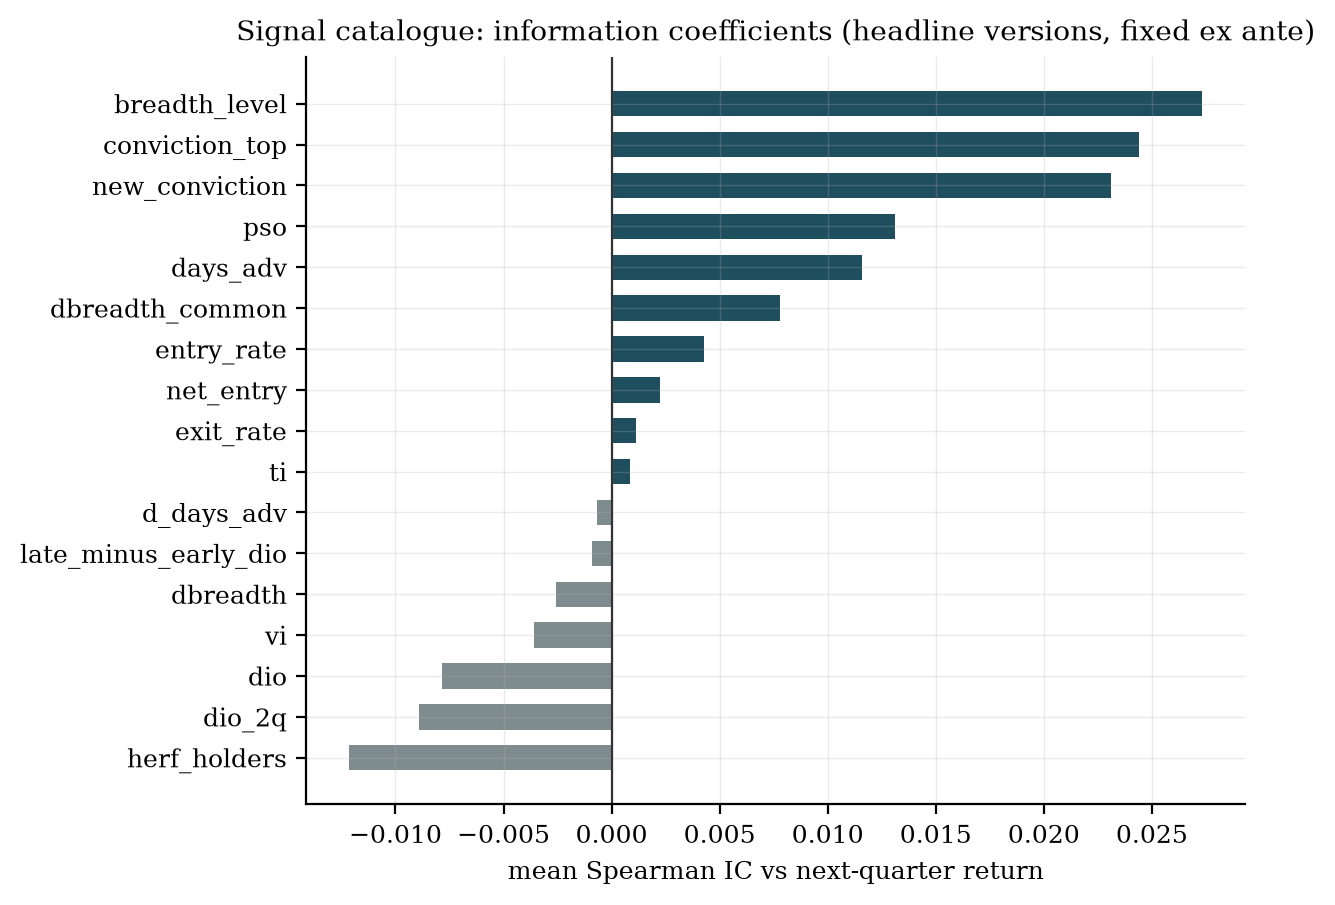
\includegraphics[width=.8\linewidth]{figs/f8_ic_bars.png}
\caption{Mean Spearman information coefficients of the catalogue
(headline versions, fixed ex ante). The conviction family leads;
state variables cluster at zero or negative.}
\label{fig:ic}
\end{figure}

\begin{table}[t]
\centering\footnotesize
\caption{Signal catalogue, headline versions, 49 event quarters.
Spread is the EW Q5$-$Q1 quarterly spread; $t$ is Newey--West;
``resid'' marks signals whose headline is the size/liquidity residual
by the ex-ante placebo rule.}
\label{tab:catalogue}
\begin{tabular}{llrrrrr}
\toprule
signal & version & spread/q & $t$ & Sharpe & IC & mono \\
\midrule
NCB (new\_conviction) & resid & $+0.0218$ & $+3.54$ & $1.08$ & $+0.023$ & $0.58$ \\
conviction\_top & resid & $+0.0223$ & $+2.39$ & $0.65$ & $+0.024$ & $0.58$ \\
breadth\_level & resid & $+0.0193$ & $+1.48$ & $0.36$ & $+0.027$ & $0.55$ \\
late\_minus\_early\_dio & raw & $+0.0068$ & $+1.24$ & $0.34$ & $-0.001$ & $0.53$ \\
entry\_rate & raw & $+0.0134$ & $+1.23$ & $0.36$ & $+0.004$ & $0.57$ \\
dbreadth\_common & raw & $+0.0049$ & $+1.07$ & $0.27$ & $+0.008$ & $0.50$ \\
exit\_rate & raw & $+0.0112$ & $+0.89$ & $0.24$ & $+0.001$ & $0.54$ \\
turnover imbalance & raw & $+0.0031$ & $+0.56$ & $0.13$ & $+0.001$ & $0.51$ \\
value imbalance & raw & $+0.0016$ & $+0.37$ & $0.09$ & $-0.004$ & $0.53$ \\
net\_entry & raw & $+0.0019$ & $+0.33$ & $0.07$ & $+0.002$ & $0.51$ \\
dbreadth & raw & $+0.0022$ & $+0.32$ & $0.06$ & $-0.003$ & $0.53$ \\
$\Delta$days-ADV & resid & $+0.0016$ & $+0.28$ & $0.06$ & $-0.001$ & $0.51$ \\
days-ADV & resid & $-0.0066$ & $-0.41$ & $-0.12$ & $+0.012$ & $0.50$ \\
pct.\ shares held & raw & $-0.0068$ & $-0.74$ & $-0.19$ & $+0.013$ & $0.52$ \\
$\Delta$inst.\ ownership & raw & $-0.0041$ & $-0.76$ & $-0.22$ & $-0.008$ & $0.45$ \\
holder Herfindahl & resid & $-0.0048$ & $-1.09$ & $-0.29$ & $-0.012$ & $0.47$ \\
$\Delta$IO (2q) & raw & $-0.0083$ & $-1.89$ & $-0.46$ & $-0.009$ & $0.48$ \\
\bottomrule
\end{tabular}
\end{table}

\subsection{Replications, stated as such}
\label{sec:replications}

We list the replication record in one place because it calibrates
trust in the new results. \citet{chs2002} breadth: replicated.
\citet{gompers2001} ownership level: the level effect does not
survive size control in the modern sample, consistent with the
mechanism being institutional \emph{flows} into preferred
characteristics rather than the level itself. Days-of-ADV
(\citet{chincarini2020} and related): raw point replicated, removed
by residualization. \citet{agarwal2013} confidential holdings: not
replicated on 2013--2025. \citet{miori2022} position-imbalance
reversal: evaluated in its oracle form and after bias correction
(Section~\ref{sec:tactical}); the adjusted premium is materially
smaller. \citet{coval2007}: the mechanism (redemption-driven selling)
replicates with $t=+20.9$; the expected-flow \emph{forecasting}
construction does not transfer to 13F-implied flows
(Section~\ref{sec:fss}). \citet{kps2019} IPCA and the bootstrap
selection protocol of \citet{oliveira2025} are applied as
methodology, each with its own verdict.

\section{New-Conviction Breadth (NCB)}
\label{sec:ncb}

\subsection{Mechanism}

A 13F reveals almost nothing about why a position exists --- except
in one corner. When a manager \emph{opens or materially grows} a
position that lands in the \emph{top decile of their own book}, the
filing records an action with three properties: it was expensive
(top-decile room is made by displacing existing conviction), it was
deliberate (indexing, rebalancing, and inflows do not create fresh
top-of-book positions), and it is comparable across managers (each
book's own weight distribution defines its threshold). NCB counts,
per stock and quarter, the fraction of filers that took this action:

\[
\mathrm{NCB}_{i,t} \;=\; \frac{1}{N_t}\,\#\Bigl\{m :\;
w_{m,i,t}\ \ge\ q_{0.90}(w_{m,\cdot,t}),\;\;
s_{m,i,t}\ \ge\ 1.25\, f_{i,t}\, s_{m,i,t-1}\Bigr\},
\]

where $w$ are within-book weights, $s$ share counts, and $f_{i,t}$ a
per-instrument split factor estimated from the holders themselves:
the modal share ratio across a stock's continuing holders identifies
splits exactly (untouched holders' ratios all land on the split
atom), validated 6/6 on prominent splits. The detector's
false-positive rate has not been separately audited; its thresholds
are deliberately conservative (modal ratio at least 15\% away from
one, held by 10\%+ of continuing holders or 30+ filers with
$2.5\times$ dominance over the runner-up atom), so the failure mode
is a missed split --- which surfaces as an outlier position change
--- rather than a fabricated one. Split adjustment matters
because unadjusted splits are \emph{differential} contamination ---
they fabricate ``buys'' precisely in the names that moved most ---
unlike ETF contamination, which is uniform and measured innocuous
(Section~\ref{sec:universe}).

The dart-throwing placebo fires for NCB (uninformed value-weighted
books mechanically open more new positions in large liquid names), so
the headline is the cross-sectional residual on $\log$ market cap and
$\log$ dollar ADV, re-ranked. The stock-level universe is every name
with at least five holders, \emph{including zero-vote names} ---
evaluating only voted names was an early bug worth recording, since
the zeros carry the sort's information too.

\subsection{Results and replications}

On the expanded universe, 2013Q3--2025Q4: quintile spread
$+1.9\%$/quarter, $t=+3.44$, Sharpe $\approx 1.0$, IC $+0.023$.
Across two universes (pre- and post-coverage-fix) and four
independent implementations (catalogue spec, standalone module,
interaction-module replication, engine panel), the $t$-statistic
lands in a $3.3$--$4.0$ band eight times. These are
\emph{implementation replications} --- robustness to construction
and coding choices on the same data, not independent samples --- and
are claimed as exactly that. The signal survives two random
50\%-coverage halvings ($t=+3.45/+2.79$). Attribution
against market, size, momentum, reversal, and illiquidity factors
leaves the premium intact (the joint Fama--MacBeth $\lambda$ of
Section~\ref{sec:fm}, $t=+3.04$ holding nine other characteristics,
is the strictest version of this statement), and no IPCA latent
factor instrumentable by the ten characteristics absorbs it
(Section~\ref{sec:ipca}).

\subsection{Hyperparameters: an a-priori spec and a measured surface}
\label{sec:ncb-surface}

The specification (book-weight quantile $0.90$, growth $1.25$,
minimum holders $5$) was fixed a priori and was the only combination
ever run during the research phase --- the eight replications carry
no tuning bias. A bootstrap-robust selection study in the
\citet{oliveira2025} protocol then mapped the full $4\times3\times3$
surface: in-sample 2013--2020, coupled moving-block bootstrap
(block~4, $B=2{,}000$, common resample indices across configurations),
selection on the 5th percentile of the bootstrap Sharpe, frozen and
evaluated 2021--2025. Three findings
(Figure~\ref{fig:surfaces}, left; full table in
Appendix~\ref{app:surfaces}):

\begin{enumerate}
\item \textbf{The surface is uniformly positive out-of-sample}: all
  36 configurations post OOS Sharpe between $+1.05$ and $+2.53$
  (every OOS $t \ge 3.2$). The default sits mid-surface; the signal
  is not fragile to its parameters.
\item \textbf{The gradient is monotone toward sharper conviction}
  (higher weight quantile, higher growth bar), in-sample and
  out-of-sample --- mechanism-consistent, and implying the a-priori
  default was conservative. The sharper corner is a post-hoc
  candidate under the funnel rules, not a new specification.
\item \textbf{An honest null on the selector}: the robust
  5th-percentile statistic picked the same configuration as the naive
  in-sample maximum and ranked the OOS ordering slightly worse
  (rank correlation $+0.41$ vs $+0.53$); at thirty in-sample
  quarters the percentile tracks the point estimate. The bootstrap's
  contribution here is distributional context (even the default's 5th
  percentile is non-negative), not selection.
\end{enumerate}

\subsection{A machine-learning cross-check that found the same thing}
\label{sec:ml}

As an ex-post exercise, we trained ridge, $k$-NN, random-forest and
gradient-boosted regressors on the twelve change-class variables to
predict the next quarter's market- and size-residualized excess
return (cross-sectional rank $z$-score target; per-quarter
winsorize/z-score features; strictly expanding walk-forward). Every
architecture predicts the size-hedged cross-section out-of-sample
($t=+2.6$ to $+3.4$ on the residualized target) --- and the exercise
is a third independent route to the same conclusion: NCB alone beats
the twelve-variable model ($+3.12\%$/q, $t=+3.50$ vs $+2.45\%$/q,
$t=+3.18$; paired $t=-1.09$); the prediction is $0.52$
rank-correlated with NCB; orthogonalized to NCB the model retains
nothing ($t=+0.40$); and the boosting's own permutation importance
ranks NCB first by a factor of three. There is no nonlinear premium
(boosted-minus-ridge paired $t=+0.27$): the linear production model
of Section~\ref{sec:fm} already extracts what exists. The exercise
also yields a practical lesson: evaluated on \emph{raw} returns the
same predictions lose money --- the prediction inherits a small-cap
exposure from the raw count features, and in a mega-cap regime that
exposure dominates. Positioning factors must be traded size-hedged;
NCB's residualized construction does this by design.

\section{Forced-Sale Supply (FSS)}
\label{sec:fss}

\subsection{The flow instrument}

For each filer, implied quarterly flow separates client/leverage
money from market growth of the book:
\[
\mathrm{flow}_{m,t} \;=\; \frac{\mathrm{AUM}_{m,t}}{\mathrm{AUM}_{m,t-1}}
\;-\;\bigl(1 + r^{\text{book}}_{m,t}\bigr),
\]
with $r^{\text{book}}$ the frozen prior book marked on the price
panel. The instrument is validated against subsequent \emph{behavior},
not returns: managers with $\mathrm{flow} < -10\%$ sell 34.5\% of
held shares over the next quarter versus 23.1\% for managers with
positive flow ($t=+10.6$; the contrast against the strictest healthy
definition reaches $t=+20.9$). Completer books strengthened the
instrument (the campaign of Section~\ref{sec:campaign}), as a real
instrument should. Selling by distressed managers is approximately
pro-rata across the liquidity spectrum (liquidity-ordering
correlation $-0.02$): the folklore ``they sell the liquid names
first'' is not in this data.

\subsection{Threshold justification without selection}

The $-10\%$ cut was set a priori. Its justification is the
\emph{shape} of the mechanism, which involves no selection at all:
the sold-fraction delta versus healthy managers rises smoothly
through every threshold --- $+7.8$pp at $-5\%$, $+11.4$pp at
$-10\%$, $+13.9$pp at $-20\%$, each with $t$ between $+9.6$ and
$+11.4$ (Figure~\ref{fig:mechanism}). The default is a point on a
monotone curve, chosen where purity meets sample size (144 distressed
managers per quarter, versus 65 at $-20\%$).

\begin{figure}[t]
\centering
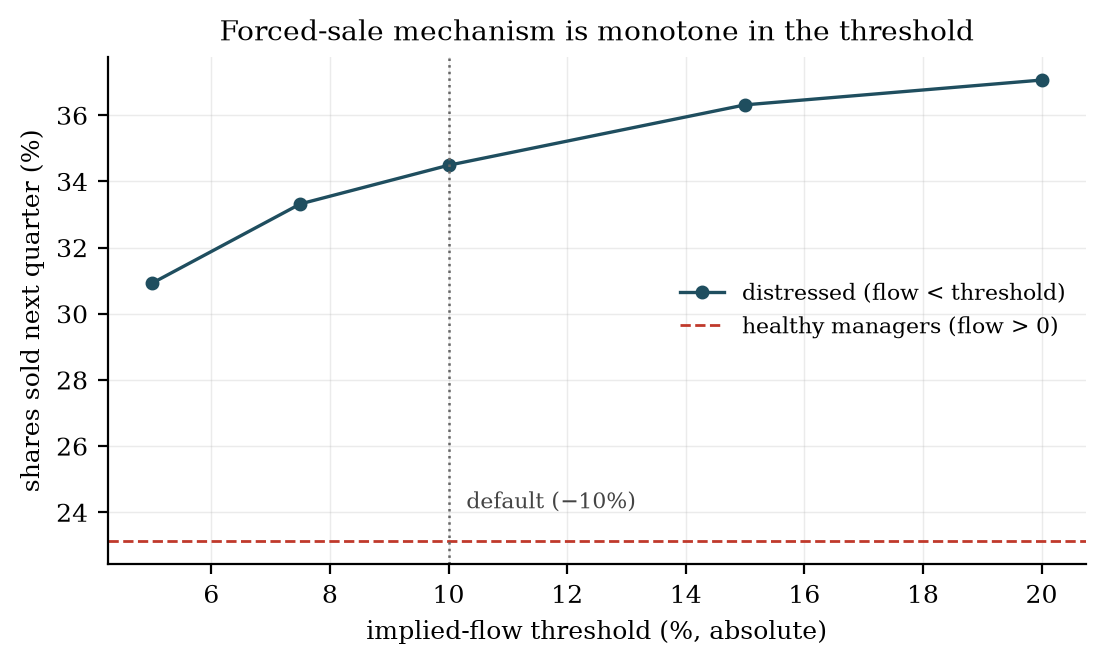
\includegraphics[width=.6\linewidth]{figs/f6_mechanism.png}
\caption{The forced-sale mechanism is monotone in the flow
threshold; the a-priori default is not a knife edge. No returns are
involved in this figure.}
\label{fig:mechanism}
\end{figure}

\subsection{From managers to stocks, and what the price says}

Stock-level supply aggregates each distressed manager's
prospective liquidation over average daily dollar volume:
$\mathrm{FSS}_{i,t}=\sum_{m \in \mathrm{dis}}
|\mathrm{flow}_{m,t}|\,\mathrm{AUM}_{m,t}\, w_{m,i,t} /
\mathrm{ADV}_{i,t}$. Pricing this basket honestly required a
benchmark audit that we report as a finding in its own right. Against
the universe \emph{mean}, the basket ``underperforms'' by
$3.8\%$/quarter --- but so does nearly everything: the cross-sectional
mean of quarterly stock returns sits $\sim$4\%/quarter above the
median through small-cap skewness, and early internal notes quoting a
$-4.5\%$/quarter cohort effect against the mean overstated the alpha.
Against the median the basket is flat. The tradable statement is the
index-hedged one: approximately flat 2013--2020 (Sharpe $-0.1$ to
$-0.5$ across all fifteen threshold$\times$basket configurations) and
\textbf{paying $+0.6$ to $+1.0$ Sharpe in 2021--2025} ($t$ up to
$+4.0$) at \emph{every} point of the grid. The grid moves as one
block: no configuration is special, none is fragile, and what the
surface identifies is a \emph{regime} --- the degrossing/rates era
--- rather than a hyperparameter.

The same surface furnishes a methodological result we consider as
valuable as the factor itself: the in-sample-to-out-of-sample rank
correlation across configurations is \emph{negative} ($-0.81$ for
the bootstrap 5th-percentile statistic). Under a regime flip, any
in-sample selector --- robust or naive --- is anti-informative. The
\citet{oliveira2025} machinery assumes a stationary utility
distribution; NCB's surface satisfies it (rank correlation $+0.53$)
and selection works there; FSS's does not, and the correct use of the
protocol is to refuse to select and report the regime
(Figure~\ref{fig:surfaces}, right). We apply our tools critically or
not at all.

\subsection{Prediction fails at every clock (Law 2)}

Three designs tried to move FSS from observation to anticipation, and
all failed their mechanism gates, which is why the production leg
reacts to filings rather than front-running them.
(i) \emph{Quarterly flow forecasting} in the \citet{coval2007}
expected-flow form (lagged flow + performance + convexity, expanding
coefficients): 13F-implied flow has no one-quarter-ahead
predictability (OOS rank correlation $-0.015$, $t=-1.21$);
predicted-distressed managers do not sell more than predicted-inflow
managers ($t=+0.69$, against $t=+20.9$ contemporaneous). The
literature forecasts \emph{reported} mutual-fund TNA flows;
13F-implied flow adds leverage, unreported assets, and frozen-book
error, which destroys the autocorrelation. (ii) \emph{Daily
synthetic stress}: retracted (Section~\ref{sec:campaign}).
(iii) \emph{Single-name crash cascades}: the middle link (salient
position crash $\to$ next-quarter redemption) does not clear its
bar ($t=-1.47$); redemptions respond to aggregate performance, which
the flow instrument already captures contemporaneously.

\section{Combining models and net-of-cost production results}
\label{sec:models}

\subsection{The Fama--MacBeth production combiner}
\label{sec:fm}

The production question --- one ranking merging the surviving 13F
signals with classical characteristics --- was raced across three
combining schools on identical quarters, strictly out-of-sample
(expanding estimates, twelve-quarter warm-up). Predictors,
pre-registered: size, momentum, beta, low-volatility, short-term
reversal, liquidity, plus NCB, breadth change, FSS, and flow
pressure, all as centered cross-sectional percentile ranks.

\begin{itemize}
\item \textbf{A. Fama--MacBeth/Lewellen} (per-quarter cross-sectional
  OLS premia, expanding mean, $E[r]=\bar\lambda'x$): spread
  $+5.4\%$/q ($t=+2.65$), \textbf{Sharpe 0.86}, IC $+0.030$.
\item \textbf{B. IC-weighted composite} (Grinold--Kahn): $+4.3\%$/q,
  Sharpe 0.69 --- univariate weights ignore signal overlap.
\item \textbf{C. Naive rank average} (NCB $+$ FSS only): $+2.6\%$/q,
  Sharpe 0.74. Paired deltas: A$-$B $t=+1.18$; A$-$C $t=+1.96$.
\end{itemize}

The joint-marginality table is the deliverable the one-at-a-time
factor ladder cannot produce: holding all ten predictors
simultaneously, NCB's premium is $t=+3.04$ and breadth change's
$t=+4.01$ --- the 13F premia are marginal to six classical
characteristics at once. Breadth change is the canonical example of
an \emph{ingredient}: weak as a standalone quintile sort
(Table~\ref{tab:catalogue}) yet the second-strongest joint premium;
signals correlated with controls reveal their value only in the
joint estimate. Figure~\ref{fig:race} shows the race cumulatively.

\begin{figure}[t]
\centering
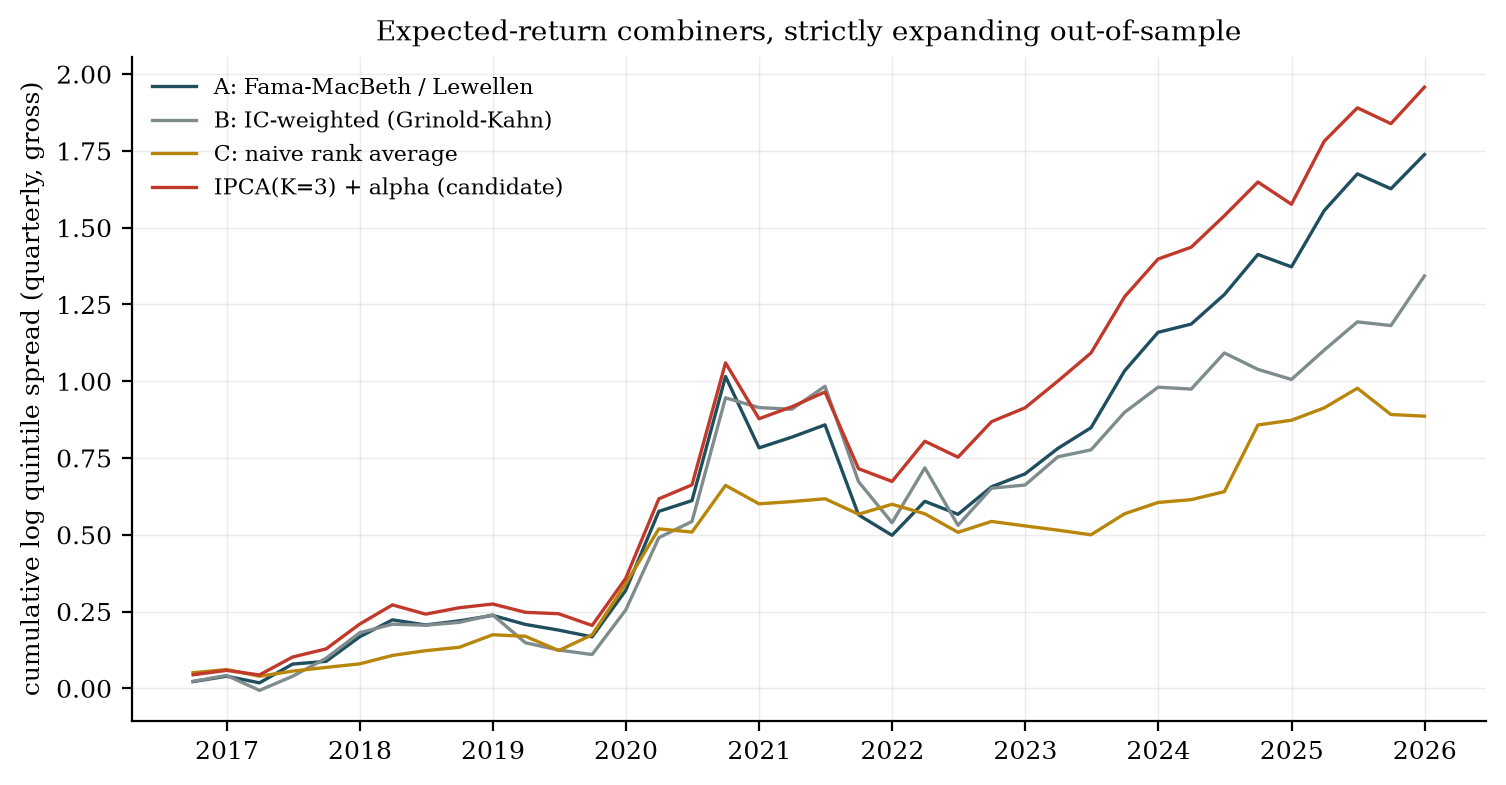
\includegraphics[width=.85\linewidth]{figs/f2_combiner_race.png}
\caption{Expected-return combiners, strictly expanding OOS, gross
quintile spreads (log cumulative). The Fama--MacBeth combiner is the
production model; the IPCA challenger is a candidate under the
funnel's promotion rules.}
\label{fig:race}
\end{figure}

\subsection{The IPCA challenger: is the premium a latent-factor loading?}
\label{sec:ipca}

Under \citet{kps2019}, factor loadings are instrumented by
characteristics ($\beta_{i,t}=z_{i,t}'\Gamma$) and estimated jointly
with latent factors by alternating least squares; our implementation
was verified line-by-line against the authors' reference package
($N_t$-weighted $\Gamma$ step, intercept as pre-specified factor,
$W_\alpha$ wild bootstrap with $t(5)$ multipliers, 500 draws). Fifty
quarters, instruments $=$ constant $+$ the ten predictors. Results:
total $R^2$ 0.10--0.12 at $K=1..4$; the formal $W_\alpha$ test does
not reject $\Gamma_\alpha=0$ ($p=0.41$--$0.59$ --- expected at
$T=50$; the test needs hundreds of periods for power); the
interpretable spanning statistic --- the time-series alpha of the
NCB-managed portfolio on the latent factors --- is $t\approx+6$ at
every $K$. Out-of-sample, the unrestricted forecast
$z'(\Gamma_\beta\bar\lambda + \Gamma_\alpha)$ posts Sharpe 0.97 and
beats the FM combiner paired ($+0.55\%$/q, $t=+2.08$); the genuinely
rank-restricted forecast ($z'\Gamma\bar\lambda$) ties FM
($t=-0.75$).

Two disciplines govern the reading. Algebraically, the unrestricted
unconditional forecast is \emph{not} rank-compressed
($\Gamma_\alpha$ is a free vector, so
$\Gamma_\beta\bar\lambda+\Gamma_\alpha$ spans $\mathbb{R}^{11}$): the
gain over FM comes from a different, pooled, structure-regularized
estimator of the same premia --- not from ``compression keeping the
alpha,'' and the leg that is genuinely compressed confirms this by
not beating FM. Procedurally, IPCA entered after the race was
scored: a post-hoc fourth entrant at $t=+2.08$ does not clear the
pre-registered promotion bar ($2.57$), so \textbf{FM remains the
production combiner} and IPCA+alpha is recorded as the best point
estimate on the protocol, pending fresh sample. What survives
unconditionally is the answer to ``is NCB beta in disguise?'': no
latent factor instrumentable by these characteristics absorbs it.

\subsection{The net engine}
\label{sec:engine}

Research spreads are gross and frictionless by construction; the
engine is neither. Every panel --- survivors and rejected signals
entered \emph{inverted}, so a positive net Sharpe means ``the
research conclusion pays'' --- runs through one realistic long-short
book: tradability filters (\$4 price, \$5M median dollar volume, 252
days of history), 20\% tails with a 40-name minimum per leg,
rebalanced at each signal's own decision dates, \textbf{5 bps per
side commissions} and \textbf{50 bps p.a.\ borrow on short legs},
daily net returns.

The cost assumptions are justified by the trading profile rather
than asserted. Five basis points per side is in line with realized
all-in commission-plus-spread costs for institutional trading of
liquid US equities, and this strategy is the easy case: quarterly
rebalancing (measured one-way turnover of $3$--$7\times$ per year,
Table~\ref{tab:engine}), no intraday urgency, and an explicit
liquidity control --- the tradability filter plus the per-leg
breadth minimum keeps individual positions small relative to ADV,
which is what keeps slippage beyond the flat fee second-order.
Market impact matters at scale and belongs to the capacity
discussion, not the backtest. Borrow at 50 bps p.a.\ is
general-collateral; because the FSS leg skews illiquid we report the
hard-to-borrow sensitivity: at 200 bps the FSS leg loses
$\approx1.5\%$/yr (Sharpe $0.85\to0.73$) and the combo
$\approx0.75\%$/yr (Sharpe $\approx0.9$) --- the conclusions
survive. The NCB$+$FSS book weights the two legs' ranks
\emph{equally by design}: the no-optimization default, chosen so the
production book inherits no tuned parameter; any data-driven leg
weighting would require its own surface under the
Section~\ref{sec:ncb-surface} protocol.

Table~\ref{tab:engine} reports the full battery
--- annualized net return, volatility, Sharpe, information ratio
against the hedged benchmark, maximum drawdown, Calmar, hit ratio ---
for the headline strategies on the expanded universe, and
Figure~\ref{fig:engine} the cumulative net curves. The engine
compresses everything (costs, the stricter universe, no shorting of
the illiquid tail), the ordering matches the research layer, and the
research-rejected signals inverted earn approximately zero net ---
the engine confirming, from the cost side, that the funnel's
rejections were correct.

\begin{table}[t]
\centering\footnotesize
\caption{Production-engine results, net of 5 bps/side commissions and 50 bps p.a.\ borrow on short legs; expanded universe; tradability filters \$4 / \$5M ADV / 252d. ``cost'' is the measured annualized commission drag (net run minus zero-fee run); ``turn'' the implied one-way annual turnover (traded notional over book, per year). Research-rejected signals enter inverted, so a positive Sharpe means the research conclusion prices.}
\label{tab:engine}
\begin{tabular}{lrrrrrrrr}
\toprule
strategy & ann.\ net & vol & Sharpe & maxDD & Calmar & hit & cost (bps/y) & turn \\
\midrule
NCB (residualized) & +2.9\% & 6.7\% & +0.42 & -18.7\% & +0.15 & 51\% & 65 & 6.5x \\
FM score (10 predictors) & +4.0\% & 16.9\% & +0.24 & -62.1\% & +0.06 & 51\% & 43 & 4.3x \\
NCB+FSS book & +6.2\% & 6.0\% & +1.02 & -10.6\% & +0.58 & 53\% & 67 & 6.7x \\
FSS short leg & +10.4\% & 12.2\% & +0.85 & -26.1\% & +0.40 & 54\% & 65 & 6.5x \\
dBreadth (common filers) & +1.4\% & 11.1\% & +0.13 & -28.2\% & +0.05 & 53\% & 61 & 6.1x \\
NCB v2 (catalogue spec) & +2.6\% & 8.3\% & +0.31 & -26.2\% & +0.10 & 53\% & 50 & 5.0x \\
Conviction top (level) & +2.5\% & 12.3\% & +0.20 & -49.6\% & +0.05 & 52\% & 33 & 3.3x \\
ICA reversal & -2.1\% & 8.2\% & -0.26 & -24.7\% & -0.09 & 49\% & 51 & 5.1x \\
SSI (inverted) & -2.0\% & 9.9\% & -0.20 & -34.8\% & -0.06 & 48\% & 29 & 2.9x \\
NMF crowding (inverted) & +0.7\% & 11.9\% & +0.06 & -51.4\% & +0.01 & 53\% & 45 & 4.5x \\
\bottomrule
\end{tabular}
\end{table}

\begin{figure}[t]
\centering
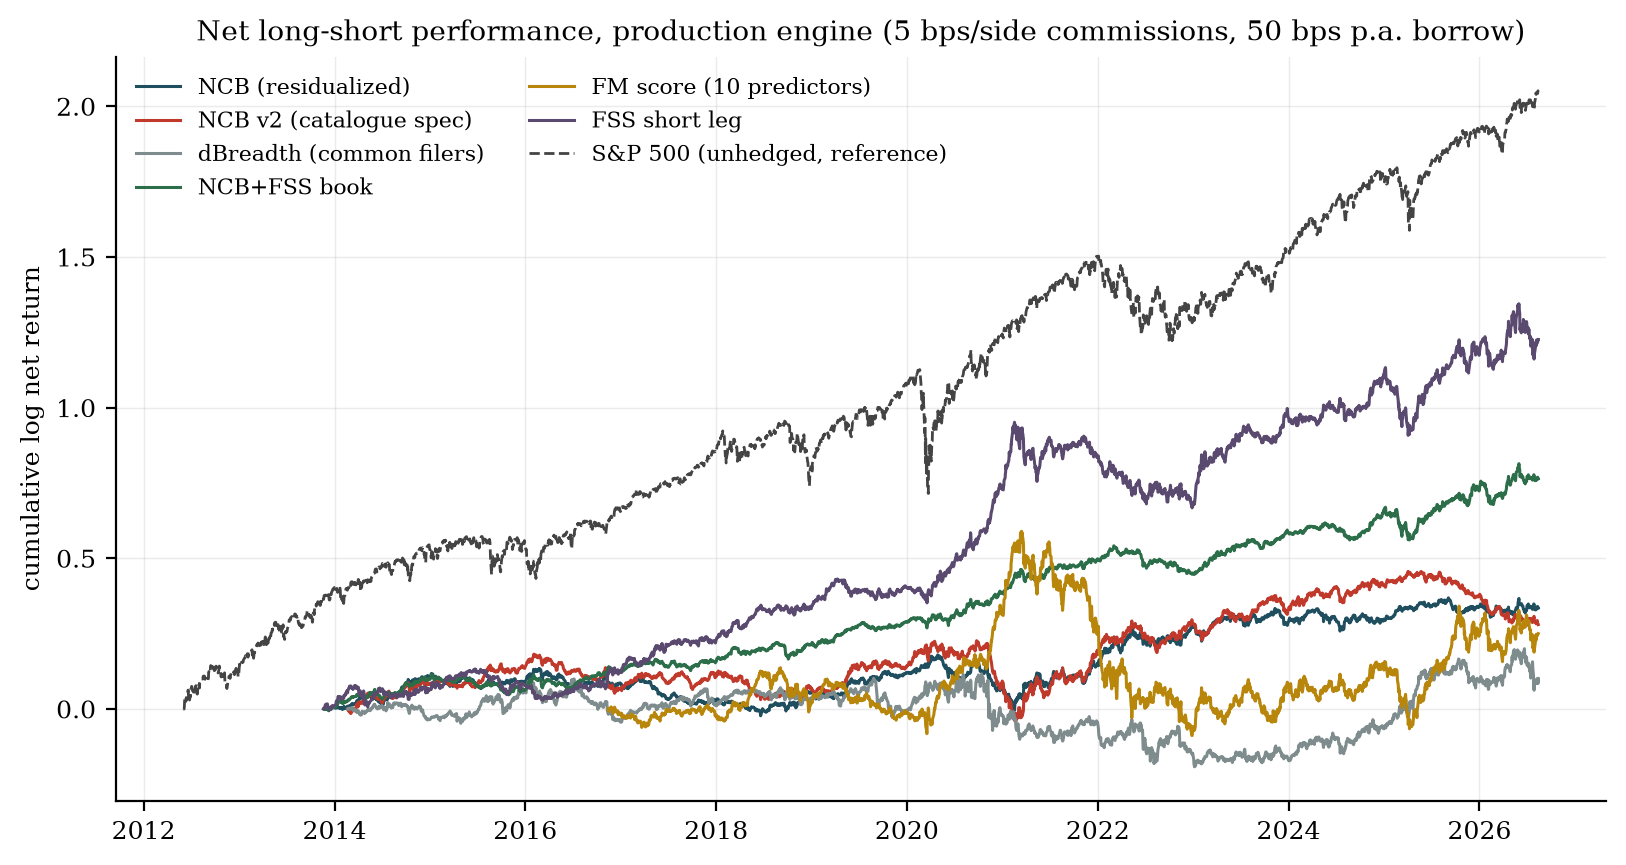
\includegraphics[width=.95\linewidth]{figs/f1_engine_curves.png}
\caption{Net long-short performance in the production engine
(log cumulative returns; 5 bps/side commissions, 50 bps p.a.\
borrow).}
\label{fig:engine}
\end{figure}

\subsection{Long-only implementation}
\label{sec:lo}

A naive long-only expression --- holding the long basket
equal-weighted against the S\&P --- is condemned by the composition
arithmetic of Section~\ref{sec:funds} before any signal question
arises: the equal-weight tilt pays the Bessembinder tax that sank
the median 13F book itself. The institutional design tilts the
\emph{benchmark}: true cap weights over the top 500 names by
repaired market capitalization (10\% cap), multiplied by
$\exp\{2k(\mathrm{rank}_i - 0.5)\}$ on the NCB$+$FSS combo rank and
renormalized, quarterly, net of 5 bps/side on turnover. The
multiplicative-exponential form is the standard tilt of
index-provider factor-tilt methodologies (MSCI-style tilt indexes
multiply parent-index weights by a positive score function): it
preserves positivity and long-only feasibility by construction,
leaves unscored names at benchmark weight (rank $0.5$), and makes
the tilt strength a single interpretable dial.
The benchmark is a genuine cap-weighted model: the top 500 names by
repaired market capitalization (official S\&P constituent weights are
licensed data; historical constituent \emph{lists} are free, weights
are not), and the repair matters --- the shares-inferred cap panel
is reliable as a ranked regression control but has a corrupt tail as
portfolio weights, fixed by replacing $|z|>2.5$ outliers of a
cross-sectional $\log(\mathrm{mcap})\sim\log(\mathrm{ADV})$
regression with their fitted values. The resulting proxy tracks the
actual S\&P~500 at a 2.7\% tracking error with $-0.6\%$/yr drift ---
close enough to serve as the cap-weighted base. Table~\ref{tab:lo}
and Figure~\ref{fig:lo}: the tilt adds $+1.0$/$+2.2$/$+3.6\%$ per
year over the benchmark at tracking errors of
$1.8$/$4.0$/$6.2\%$ for $k=1/2/3$ --- an information ratio of
$0.53$--$0.58$, \emph{roughly flat in the tilt strength}, the
signature of a scalable signal rather than a lucky corner. All three
variants also clear the S\&P itself.

\begin{table}[t]
\centering\small
\caption{Long-only cap-weighted model and its combo tilts, net of
5 bps/side commissions, quarterly rebalance, 2013--2026. ``Total
ret.'' is the portfolio's full net return (long-only, $\beta\approx
1$: it contains the market); the \emph{alpha} columns are
``excess''/IR --- against the tilt's own benchmark in the top block,
against the actual S\&P~500 in the bottom block. Rel.\ maxDD: worst
peak-to-trough of the log wealth ratio versus the same reference.
No bootstrap-selected $k$ appears \emph{by design}: the tilt-strength
surface (Figure~\ref{fig:losurface}) gives no evidence that
selecting or re-selecting $k$ from history helps, and weak evidence
that it hurts --- $k$ is shipped as the conservative default
($k=1$) and scaled by the investor's tracking-error budget.}
\label{tab:lo}
\begin{tabular}{lrrrrrrrr}
\toprule
portfolio & total ret.\ (net) & vol & Sharpe & maxDD & excess & TE &
IR & rel.\ maxDD \\
\midrule
S\&P 500 (actual index) & $+14.8\%$ & $17.1\%$ & $0.86$ & $-41.1\%$
& --- & --- & --- & --- \\
cap-weighted 500 (S\&P proxy) & $+14.1\%$ & $18.0\%$ & $0.78$ &
$-44.6\%$ & --- & --- & --- & --- \\
combo tilt $k=0.5$ & $+14.6\%$ & $18.2\%$ & $0.80$ &
$-44.6\%$ & $+0.4\%$ & $0.9\%$ & $0.49$ & $-2.5\%$ \\
combo tilt $k=1$ \textbf{(shipped default)} & $+15.1\%$ & $18.4\%$
& $0.82$ & $-44.5\%$ & $+1.0\%$ & $1.8\%$ & $0.53$ & $-5.7\%$ \\
combo tilt $k=2$ & $+16.4\%$ & $19.2\%$ & $0.85$ & $-44.1\%$ &
$+2.2\%$ & $4.0\%$ & $0.57$ & $-13.7\%$ \\
combo tilt $k=3$ & $+17.7\%$ & $20.4\%$ & $0.87$ & $-43.9\%$ &
$+3.6\%$ & $6.2\%$ & $0.58$ & $-21.2\%$ \\
\midrule
benchmark vs S\&P & & & & & $-0.6\%$ & $2.7\%$ & --- & $-17.0\%$ \\
$k=1$ vs S\&P & & & & & $+0.3\%$ & $3.6\%$ & $0.09$ & $-13.6\%$ \\
$k=3$ vs S\&P & & & & & $+2.9\%$ & $7.3\%$ & $0.40$ & $-25.5\%$ \\
\bottomrule
\end{tabular}
\end{table}

\begin{figure}[t]
\centering
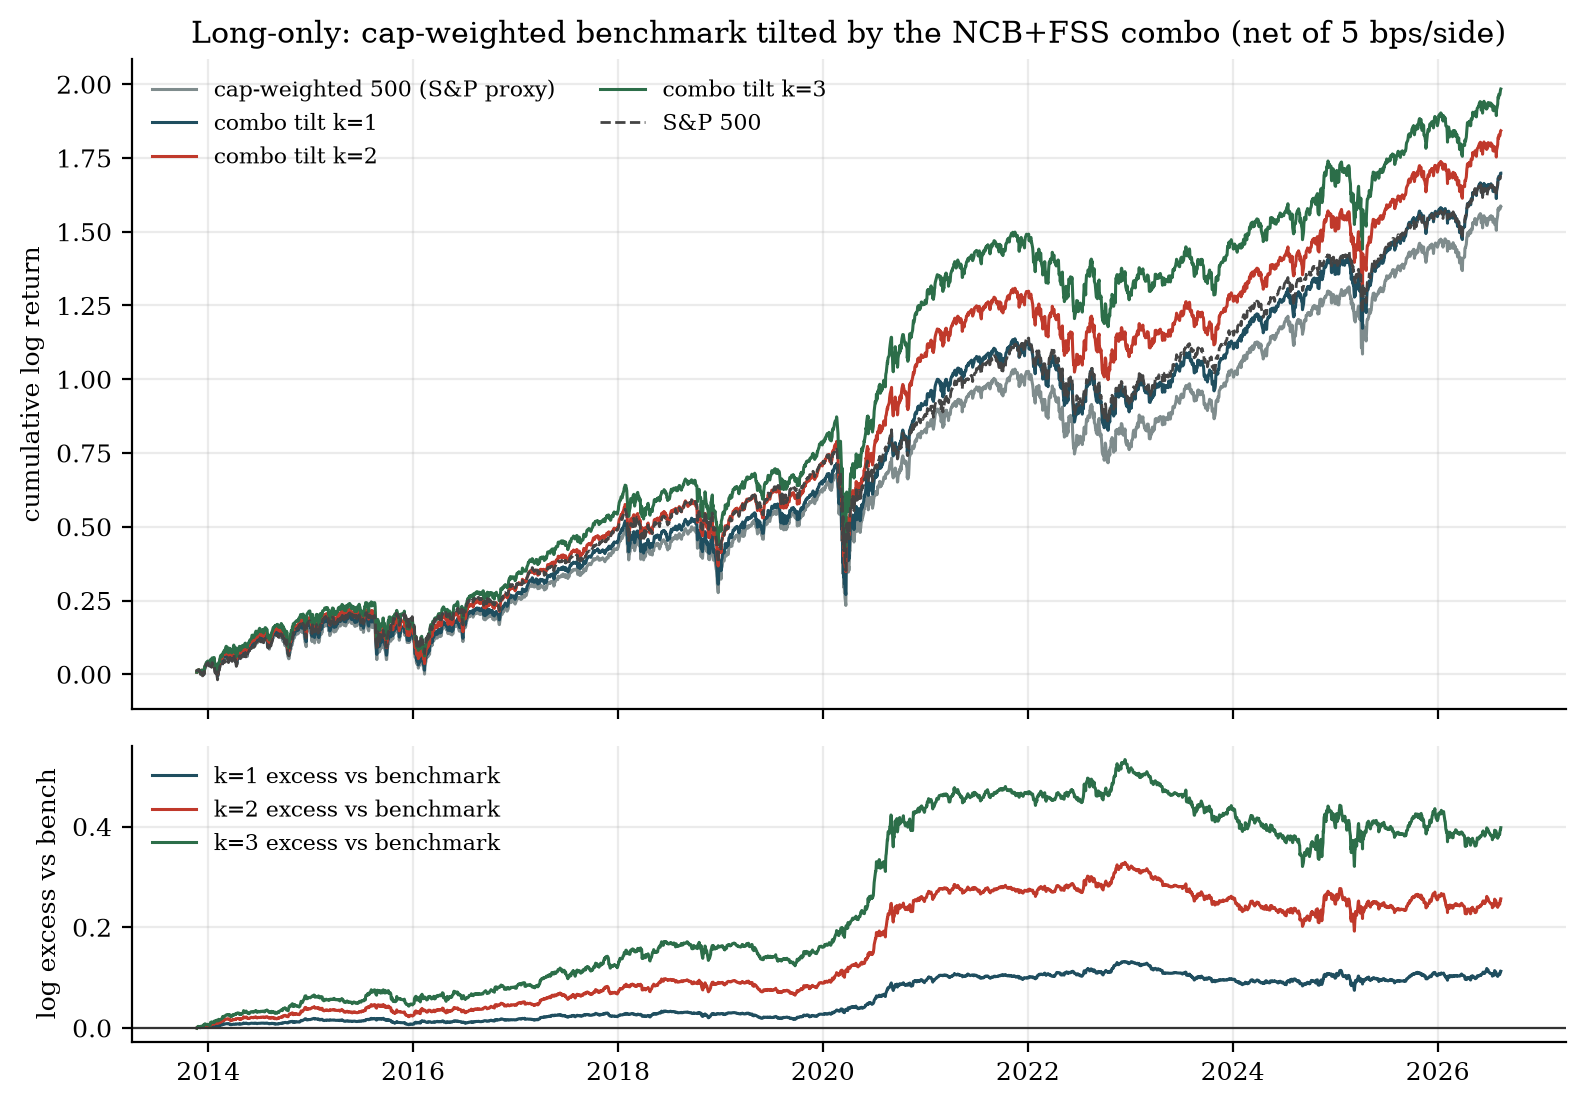
\includegraphics[width=.9\linewidth]{figs/f11_long_only.png}
\caption{Long-only benchmark tilt (log cumulative, net). Top:
levels; bottom: log excess versus the benchmark by tilt strength.}
\label{fig:lo}
\end{figure}

\paragraph{Justifying the tilt strength: the third surface.}
The one free parameter of the LO product, $k$, received the same
bootstrap treatment as the NCB and FSS specifications (grid
$k\in\{0.5,\dots,4\}$; utility $=$ IR of quarterly excess vs the
benchmark; coupled block bootstrap of the in-sample years, one IR
distribution per $k$; frozen OOS 2021--2025).
Figure~\ref{fig:losurface}: in-sample the distributions shift up
with $k$ (median IR $0.59\to1.09$; even the 5th percentile turns
positive from $k=1$) --- and in the held-out years the ordering
reverses (IR $0.42$ at $k=0.5$ down to $-0.04$ at $k=4$). Two
honesty caveats size this correctly. First, with 23 held-out
quarters the standard error of an annualized IR is $\approx 0.4$,
so the reversal is \emph{suggestive, not proven}. Second, the
mechanism is mundane: the exponential tilt is nonlinear --- large
$k$ concentrates the book far from cap weights, degrading the
transfer coefficient per unit of tracking error, and the 2021+
mega-cap regime taxed exactly that deviation. The natural objection
--- ``why not re-select $k$ each period with an expanding window?''
--- was simulated directly: an adaptive selector maximizing
expanding-window IR picks $k=4$ in essentially every quarter from
2015 through 2022 (in-sample always rewards aggression), which makes
it approximately equivalent to holding the most aggressive tilt
throughout; it earns $-0.11$ after 2021 against $+0.31$ for the
frozen default. The defensible statement is deliberately modest:
\textbf{there is no evidence that re-selecting $k$ helps, weak
evidence that it hurts, and since large $k$ buys tracking error
without reliable additional excess, the shipped default is the
conservative $k=1$} --- with $k$ treated as the investor's
tracking-error budget ($0.9\%$ at $k=0.5$, $1.8\%$ at $k=1$, $6\%$
at $k=3$), not as a fitted parameter.
Across the three applications of the \citet{oliveira2025} protocol,
one surface supported selection (NCB: IS ranks OOS at $+0.53$) and
two refused it (FSS $-0.81$, LO tilt $-1.0$) --- the protocol's
value in this project was less in picking parameters than in
\emph{detecting when picking is illegitimate}.

\begin{figure}[t]
\centering
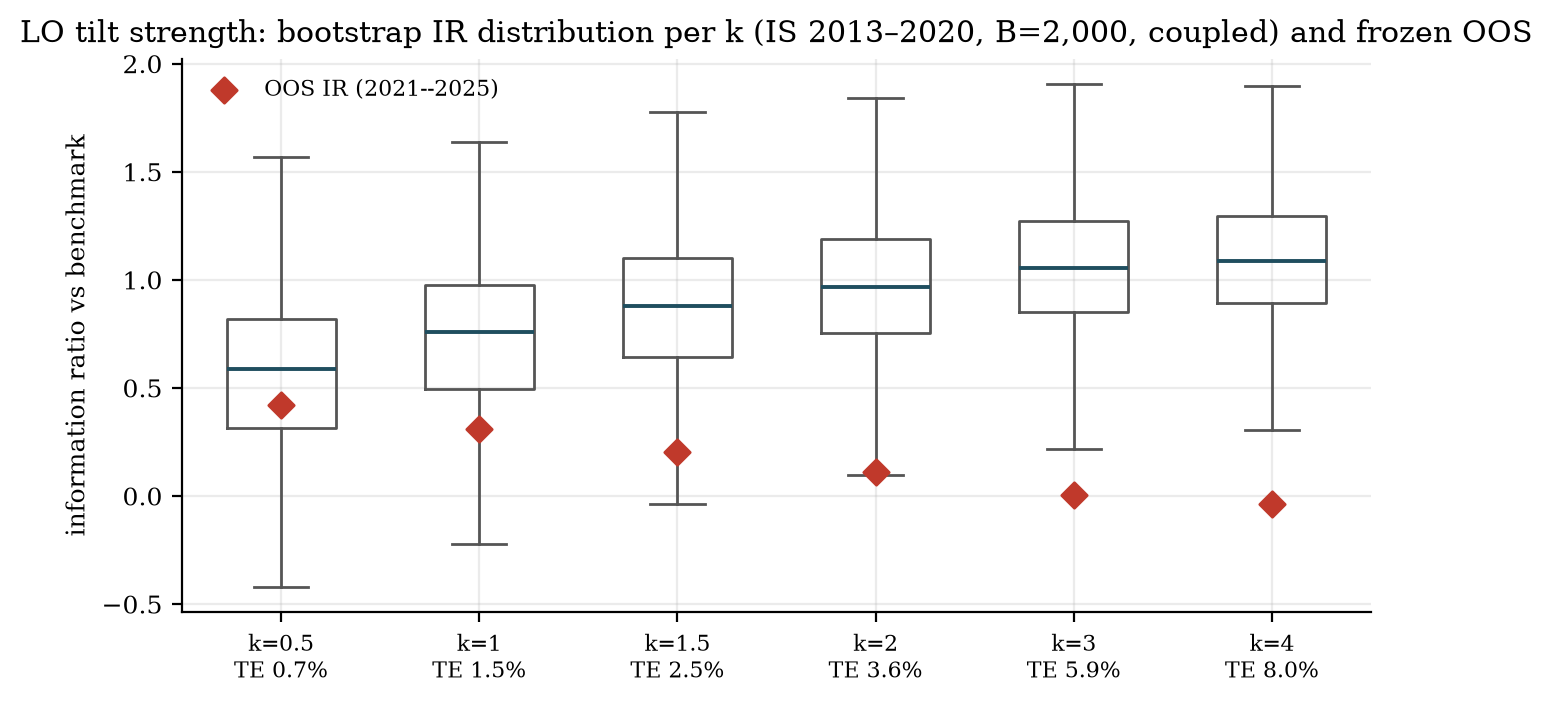
\includegraphics[width=.8\linewidth]{figs/f12_lo_surface.png}
\caption{One bootstrap IR distribution per tilt strength (boxes:
in-sample 2013--2020, coupled resamples) against the frozen held-out
IR (diamonds). The in-sample ordering reverses in the held-out years
--- suggestive at this sample size (IR s.e.\ $\approx 0.4$), and
enough to treat the tilt strength as a risk budget rather than a
fitted parameter.}
\label{fig:losurface}
\end{figure}

\paragraph{The research-to-production decomposition of the FM
combiner.} The FM combiner's research Sharpe (0.86, gross quintile
spreads on the wide $\ge$5-holder universe) does not survive the
engine (net Sharpe 0.24, $-61\%$ drawdown), and the decomposition is
a result in itself, produced by three controlled cuts. Costs are
irrelevant (0.24 with commissions, 0.26 without). The engine is
faithful (a plain quintile spread of the same ranking on the engine's
tradable universe reproduces the engine's Sharpe). What kills it is
composition: on the tradable universe the raw ranking retains
$+2.2\%$/q (Sharpe 0.41, $t=+1.32$), and residualizing the ranking
on size and liquidity leaves \emph{nothing} ($-1.1\%$/q, $t=-0.70$).
The combiner's headline premium rides its two largest lambdas ---
size ($t=+4.45$) and liquidity ($t=+4.39$) --- which pay either
outside the tradable set or as risk compensation the engine cannot
monetize. The tradable alpha inside the ranking is precisely its 13F
components, which is why the production book is NCB$+$FSS
(Table~\ref{tab:engine}: net Sharpe \textbf{1.03}, maximum drawdown
$-11\%$) rather than the full ten-characteristic ranking. The joint
FM machinery keeps its role as the \emph{measurement} device
(Section~\ref{sec:fm}); the tradable book is built from the
components that survive on the tradable universe.

\section{Latent structure: ICA on flows, NMF on portfolios}
\label{sec:latent}

\subsection{Why ICA and not PCA, from the data up}

The starting object is a panel: rows are quarters, columns are
managers, cells are the validated implied flow of that manager in
that quarter. Individual flows are not independent --- common
currents run behind them (hedge-fund redemption waves, rotation to
passive, the 2020 panic) --- and we want the currents separated. The
situation is the cocktail-party problem: each manager is a microphone
recording a mixture of conversations, and nobody hands you the
conversations.

PCA cannot solve it, for a reason worth being precise about. PCA uses
only covariance, and covariance is blind to \emph{shape}: a steady
$\pm$ breathing pattern and a silent-then-burst pattern with the same
variance are identical to it. Worse, for Gaussian-looking data any
rotation of the true sources reproduces the same covariance, so PCA
returns an arbitrary rotation --- a way of summing the
conversations, not the conversations. The current we care about ---
forced selling --- is precisely the bursty one: quiet for years, then
one violent quarter. Its signature lives in kurtosis and asymmetry,
not variance. ICA inverts the central limit theorem: mixing makes
things more Gaussian, so unmixing means finding the \emph{least}
Gaussian combinations. A forced-liquidation burst is the least
Gaussian object in a flow panel.

We extract $K=6$ components with expanding-window FastICA and
classify each by shape alone --- high kurtosis with low persistence
$=$ forced; smooth and persistent $=$ allocative --- never touching
returns in the classification. Three validations discipline the
construction. \emph{Rotation placebo}: applying the same trading
logic to variance-preserving rotations of the components (what PCA
would deliver) destroys the effect --- reversal thesis $t=+1.29$ on
ICA components versus $-0.77$ rotated; the information lives exactly
in the shape only ICA preserves. \emph{Unlabeled crises}: the forced
components' burst quarters land on the taper tantrum, Brexit, and
COVID without the model ever seeing a calendar. \emph{Stability}:
the identified subspace persists at 81\% quarter over quarter
(measured as subspace overlap; components may permute or flip sign
without anything real changing). The tradable edge is modest and
reported as modest --- approximately zero net in the engine --- and
the piece's value is identification: it is the cleanest demonstration
in the project that a ``sophisticated'' method can be held to placebo
and stability standards like any signal.

\subsection{NMF latent strategies}

Non-negative matrix factorization of the manager$\times$stock weight
panel yields components that are themselves long-only portfolios ---
the honest reason to prefer NMF over PCA/SVD here, since a manager is
interpretable as a mixture of strategy books but not as a sum of
axes with negative holdings. $K=10$--$12$ selected by held-out
manager reconstruction; the structure is stable across the coverage
expansion. As a crowding predictor the construction fails
(Section~\ref{sec:laws}; the conditional fragility test returns the
sign \emph{opposite} to the \citet{greenwood2011} thesis), and its
retained roles are measurement and clustering: the strategy mixtures
are the natural pooling groups for hierarchical (James--Stein)
estimation of per-manager parameters, which is where any future
flow-forecasting attempt with reported-TNA data would start.

\section{Event-clock studies, monitors, and tactical results}
\label{sec:tactical}

\paragraph{The clock itself.}
Entering each name on the day its information became public (per
holder-filing acceptance) instead of the D+45 batch adds
$+0.21\%$/yr on the long side ($t=0.18$) and $+0.31\%$/yr on the
short ($t=-0.22$): the cost of the batch clock is measured at
approximately zero, consistent with the delay distribution of
Section~\ref{sec:delays}.

\paragraph{Classical interactions: five pre-registered conditional
effects, none confirmed.}
Theory motivates conditioning each 13F signal on a classical
characteristic; five such interactions were pre-registered with
target cells, expected signs, and a Bonferroni bar of $|t|\ge2.57$
for the family. None confirmed (Table~\ref{tab:inter}); NCB
replicated unconditionally at $t=+3.78$ inside the same module ---
the factor is broad, not a corner-case effect.

\begin{table}[t]
\centering\footnotesize
\caption{Pre-registered 13F$\times$classical interactions, 50
quarters. Verdict statistic: paired delta between the target-tercile
spread and the unconditional spread, NW(4).}
\label{tab:inter}
\begin{tabular}{llrrl}
\toprule
interaction (theory) & target & uncond.\ (t) & delta (t) & verdict \\
\midrule
NCB $\times$ mktcap (limits to arbitrage) & small & $+3.78$ & $+1.34$ & not confirmed \\
dbreadth $\times$ IO (\citealt{nagel2005}-style) & low IO & $+1.17$ & $-1.42$ & not confirmed \\
FSS $\times$ ADV (impact where illiquid) & illiquid & $-0.90$ & $+1.05$ & not confirmed \\
pressure $\times$ vol (flow moves price in high vol) & high vol & $+1.09$ & $+0.77$ & not confirmed \\
exit\_rate $\times$ momentum (exodus in losers) & losers & $+0.96$ & $+2.02$ & wrong sign \\
\bottomrule
\end{tabular}
\end{table}

\paragraph{The pressure autopsy: why flow pressure should pay, why
it mostly does not, and where the lesson survived.}
The economic case for a flow-pressure factor is genuine, and its
failure is as informative as NCB's success. A 13F reveals flows that
were \emph{already executed}: by the decision date the quarter's
selling has largely happened and its price impact is realized inside
the filing quarter --- which is why the unconditional pressure
signal dies once orthogonalized to momentum, reversal, and the
concurrent quarter's return; there is nothing left to forecast. The
one situation where pressure should still pay \emph{forward} is an
\emph{unfinished liquidation}: a position large relative to ADV
cannot be unwound in one quarter, so the filing reveals pending
supply rather than consumed supply. This is measured, not
conjectured: the mechanism stage of Section~\ref{sec:fss} shows
distressed managers selling 34.5\% of remaining shares in the
quarter \emph{after} the filing --- liquidation demonstrably
continues past the disclosure.

Two conditioning routes follow, with different fates. Route one
conditions on the \emph{stock}: pressure should matter more where
volatility is high (valuation uncertainty amplifies the impact of
uninformed flow) --- the E4 interaction above, and the project's
cleanest example of a flicker dying properly: promising in smoke,
$t=+2.06$ on the old universe (just under the promotion bar), an
identification autopsy --- conditioning on residual volatility
versus ADV versus market cap to separate valuation uncertainty from
disguised illiquidity --- that returned ``exploratory, no formal
claim'' ($t=-0.50/-0.61$), and a fall to $t=+0.77$ on complete
books: non-promotion vindicated by data it had never seen. Route two
conditions on the \emph{seller}: restrict to managers whose selling
is \emph{forced}, where continuation is guaranteed by the redemption
itself rather than inferred from the stock's characteristics. That
route is FSS, and it is the one that prices. The design lesson:
\textbf{condition on the agent's constraint, not on the asset's
state} --- the same asymmetry as Law 1.

\paragraph{Imbalance reversal (\citealt{miori2022}).}
Replicated in oracle form and re-evaluated with the biases removed
(point-in-time snapshots instead of perfect foresight of the
cross-section; universe-churn control): the adjusted premium is a
fraction of the published point. We report both numbers as the
clearest example in the project of how much 13F results depend on
who-knew-what-when accounting.

\paragraph{Quarter-end effects.}
The window-dressing design (learned manager propensity, within-loser
test to kill the momentum confound, permutation placebo) rejected
both pre-registered signs, with the placebo tracking the thesis ---
whatever exists lives in ownership/ADV structure, not in
window-dressing propensity. A residual, honestly labeled
hypothesis-generating: the post-photo reversal is entirely a
December phenomenon ($-1.91\%$ in Q4 versus $-0.05\%$ otherwise,
eleven annual observations), observationally equivalent to
portfolio pumping \citep{carhart2002} or a January
low-institutional-ownership bounce; with $n=11$ it remains a
footnote.

\paragraph{Amendment events.}
Across 250k direction-signed events, material restatements move
prices \emph{against} the direction of the correction
($-0.10\%$ at $+3$d, $t=-3.52$; clean pre-event placebo);
administrative amendments are zero, as they must be; confidential
NEW-HOLDINGS reveals drift positively at $+10$d but with a
contaminated placebo. The pre-registered thesis (price follows the
correction) is dead; the inverted fact is consistent with amendments
following stale-price attention rather than creating news.

\paragraph{Daily monitors.}
Three daily rules were evaluated against pre-registered bars on the
drifted-book machinery. The short-squeeze alarm inverted into the
useful rule: shorts spiking $+7\%$/5d on doubled volume
\emph{revert} ($-1.21\%$ over the next 5d versus $-0.12\%$ calm,
$t=-2.60$) --- the anti-panic rule is to hold, not cover.
The aggregate deleveraging index is a risk conditioner, not a
signal: correlation $+0.14$ with future ten-day market volatility,
zero with future returns (Law 1 again); throttling gross above its
expanding 80th percentile improves the combo proxy's Sharpe
0.49$\to$0.55 and drawdown $-17\%\to-15\%$. Early covering at
apparent exhaustion loses $1.5\%$/quarter to save 7 bps of borrow
--- the pressure continues; the short is held through the quarter.
The post-exhaustion tactical \emph{long} died at its gate
(stress doubles the forced-sale rate, $12.2\%$ vs $6.7\%$, but the
thesis-minus-placebo event return is $t=+0.95$, and the only
significant cell is \emph{continuation}): distressed books do not
V-bounce.

\section{Context: why imitating these books is a losing design}
\label{sec:funds}

A descriptive base rate disciplines every 13F strategy discussion.
Across 1{,}597 large filers ($\ge\$1$B disclosed book,
coverage-eligible, 2013--2026), the median frozen-book excess return
against the S\&P~500 is $\mathbf{-3.3\%}$ \textbf{per year before
fees}; only 13\% of funds have a positive information ratio, and the
best IR in the universe is $\approx 1.0$. Skill persistence ---
the rank correlation of information ratios between the sample's
halves --- is $+0.25$: real but far below what manager selection
requires, and the measured root cause of the entire smart-money
graveyard (Section~\ref{sec:laws}).

The composition arithmetic matters more than the skill statement. The
cap-weighted index self-concentrates into its winners, and over this
sample a handful of mega-caps generated most of the index return
while the median stock lagged far behind \citep{bessembinder2018}.
Any portfolio more diversified than cap-weight --- and every 13F
book is, by mandate, liquidity, or prudence --- carries an
equal-weight tilt that this regime taxed structurally. The group
sorts photograph the tax directly: 27-name books lose $3.2\%$/yr
with 24\% positive-IR, while 790-name books sit at 1\%; true active
share is monotone in IR; turnover sorts favor the active. Two design
conclusions follow. A long-only-versus-S\&P imitation strategy is
condemned by arithmetic before any signal question arises. And the
alpha in this dataset lives not in the books but in the \emph{flows
and constraints between managers} --- fresh conviction and forced
selling --- exactly where the funnel found it. Caveats stated: the
disclosed book is long-only (no shorts, cash, or intra-quarter
turnover), and survivorship biases the level upward.

\begin{figure}[t]
\centering
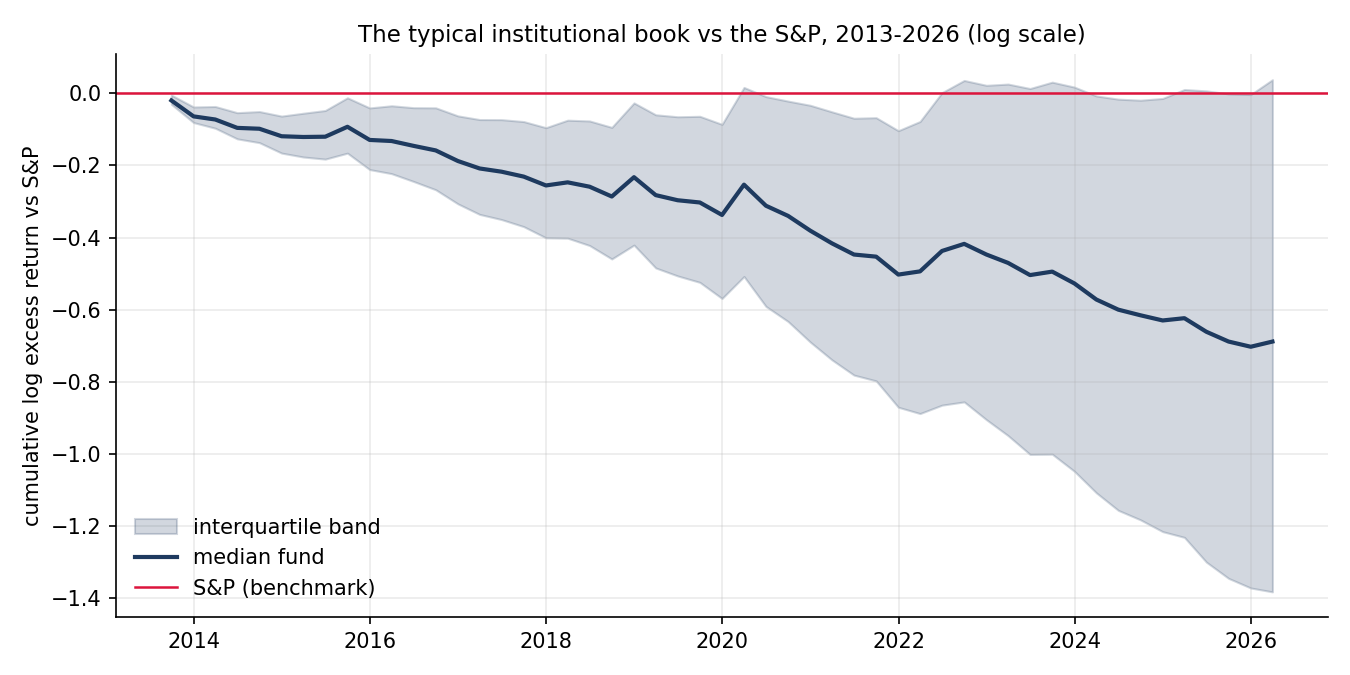
\includegraphics[width=.9\linewidth]{figs/funds_cum_log_excess.png}
\caption{Cumulative log excess return versus the S\&P~500 of large
13F filers (median and quantile bands): the median large
institutional book loses steadily against the index before fees.}
\label{fig:funds}
\end{figure}

\begin{figure}[t]
\centering
\begin{minipage}{.48\linewidth}
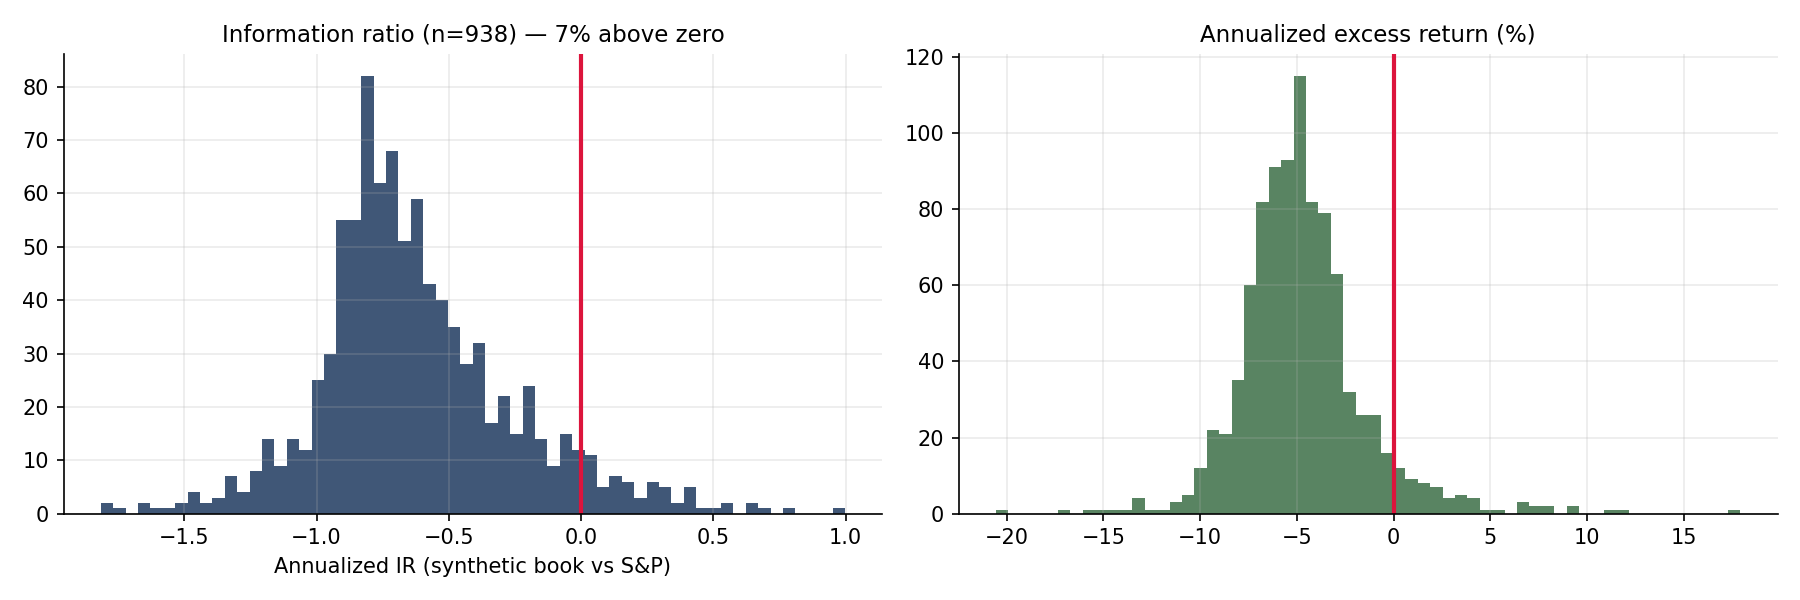
\includegraphics[width=\linewidth]{figs/funds_ir_histogram.png}
\end{minipage}\hfill
\begin{minipage}{.48\linewidth}
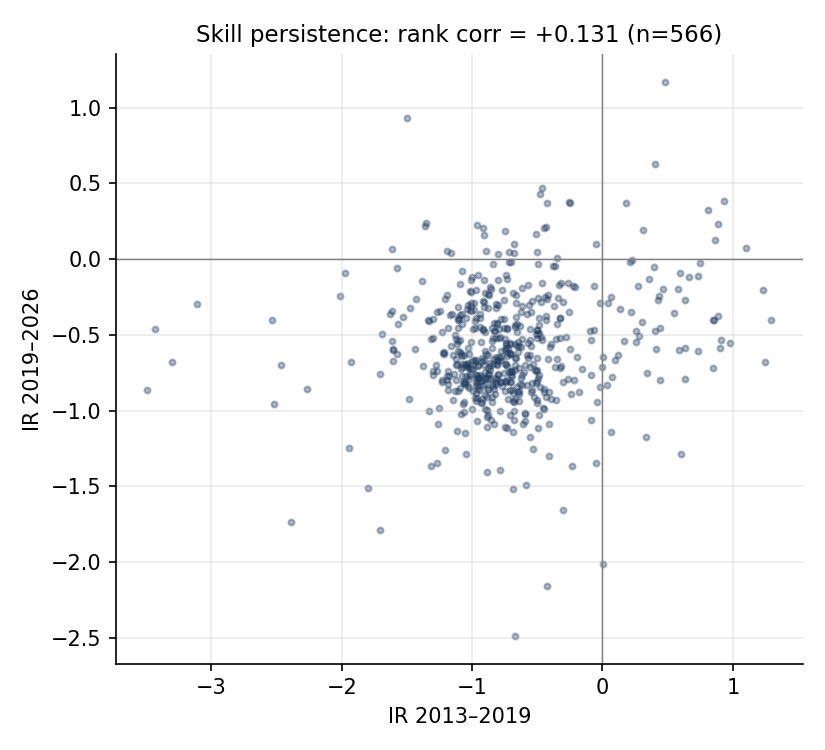
\includegraphics[width=\linewidth]{figs/funds_persistence.png}
\end{minipage}
\caption{Left: information-ratio distribution across 1{,}597 large
filers --- 13\% positive, best $\approx 1.0$. Right: skill
persistence (IR rank, first vs second half): $+0.25$, the measured
root of the smart-money graveyard.}
\label{fig:funds2}
\end{figure}

\section{The graveyard, and the two laws it obeys}
\label{sec:laws}

Negative results are reported with the same protocol as positive
ones, because the map of what fails is half the deliverable.
Table~\ref{tab:graveyard} lists every rejected design with its
verdict statistic; each has a full module report with its
pre-registration in the repository. The pattern is not random.

\paragraph{Law 1: states have no arrow.} Fifteen crowding and
ownership-state formulations --- days-of-ADV held (level and its
published value-weighted point, which replicates raw and dies
residualized), ownership share, holder concentration, institutional
ownership changes at one and two quarters, breadth level, factor
crowding from manager tilts (three hypotheses), co-ownership graph
diffusion, flow-vulnerability centrality, forced-sale absorption and
overhang, latent-strategy crowding, and the aggregate stress index
against future returns --- carry no directional information. States
earned exactly two jobs in the production stack: denominators (ADV,
AUM) and risk conditioning (the deleveraging index against future
volatility). The one crowding-adjacent object that pays, FSS, is not
a state: it is a forced action divided by liquidity.

\paragraph{Law 2: distress is information when observed, never when
predicted.} Contemporaneous: $t\approx+10$ selling contrast, the FSS
regime short, the anti-panic monitor. Predictive: quarterly flow
forecasting dead at its mechanism gate; daily stress anticipation
retracted; crash cascades gated; exhaustion longs dead. Both clocks,
both directions, one conclusion --- and it implies the production
design: react fast to filings, do not front-run them.

\begin{figure}[t]
\centering
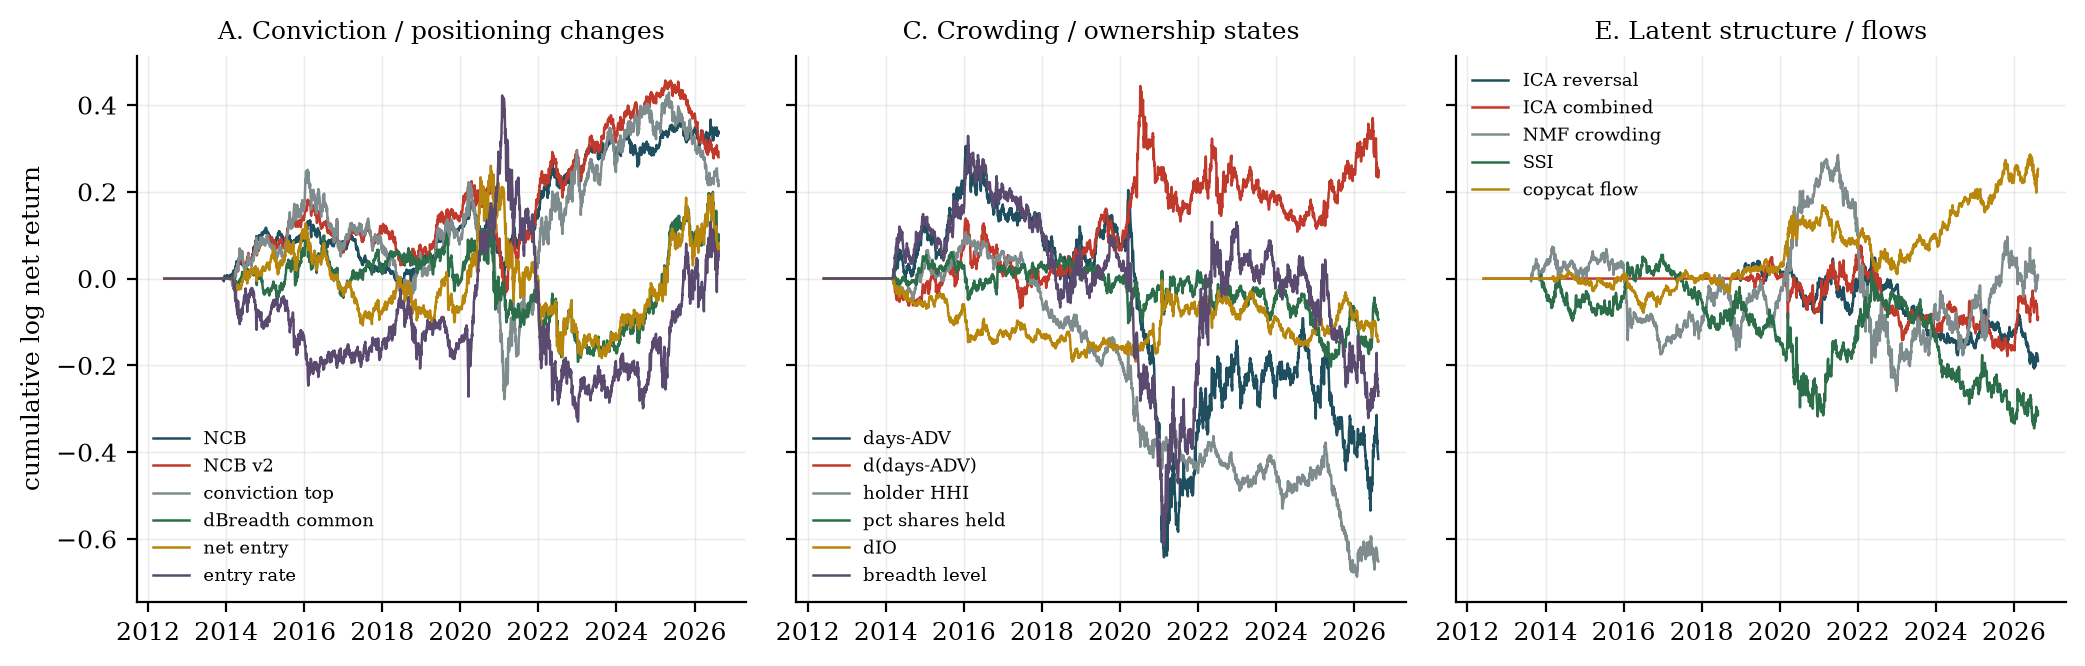
\includegraphics[width=\linewidth]{figs/f3_class_curves.png}
\caption{Net engine curves by signal class (log cumulative). The
conviction class carries the performance; the state class oscillates
around zero for a decade; the latent-structure class validates as
measurement but earns nothing net.}
\label{fig:classes}
\end{figure}

\paragraph{The smart-money corollary.} Nine designs weighting
managers by past performance or filtering the universe by manager
quality returned zero, and the base rates of
Section~\ref{sec:funds} say why: skill persistence of $0.25$ is too
weak to select on, and manager performance rank is approximately
orthogonal to \emph{which stocks} managers hold, so reweighting the
electorate reweights at random.

\begin{table}[t]
\centering\scriptsize
\caption{The graveyard. Every rejected design, its verdict statistic,
and its class. Full pre-registrations and reports in the repository
modules.}
\label{tab:graveyard}
\begin{tabular}{llll}
\toprule
design & class & verdict statistic & lesson \\
\midrule
performance-sigmoid vote weights & D & $t=+0.06$ & skill rank $\perp$ holdings \\
top-performer universes & D & negative & same \\
empirical-Bayes skill weights & D & negative & same \\
vol-scaled performance weights & D & negative & same \\
activity/concentration filters (U1--U4) & D & up to $t=-2.54$ & census beats filters \\
patient-manager universe & D & $t=-2.35/-3.25$ & same \\
follow-the-leader trading & B & hangover $t=-2.5$ & echo arrives late \\
five 13F$\times$classical interactions & A & none pass $2.57$ (5 tests) & signal is broad \\
pressure$\times$volatility (E4) & B & $t=+2.06\to+0.77$ & flicker died on fuller data \\
window dressing & F & both signs wrong & structure, not propensity \\
restatement direction-following & F & inverted ($t=-3.5$) & attention, not news \\
crash$\to$redemption cascade & B & gate $t=-1.47$ & 13F clock too coarse \\
funding-shock beta & C & $t=+0.77$, 2--3 episodes & not yet testable \\
exhaustion tactical long & F & thesis$-$placebo $t=+0.95$ & pressure continues \\
daily stress-anticipation short & F & \textbf{retracted} & eligibility artifact \\
correlation stress triggers & F & smoke mirage & Law: smoke never decides \\
cover-at-exhaustion & F & $-1.5\%$/q for 7 bps & hold the short \\
hot-ownership long warning & F & $t=+0.79$, wrong sign & --- \\
flow forecasting (stop-out prediction) & B & OOS rank-corr $-0.015$ & Law 2 \\
factor crowding as predictor & C & dead five ways & Law 1 \\
NMF strategy-crowding fragility & C & sign opposite thesis & Law 1 \\
ICA reversal as tradable & E & net $\approx 0$ & identification, not alpha \\
breadth level as factor & C & net Sharpe $-0.07$ & Law 1 \\
imbalance reversal (bias-adjusted) & F & premium shrinks & PIT accounting bites \\
ML nonlinear premium & A & boosted$-$ridge $t=+0.27$ & linear extracts it \\
\bottomrule
\end{tabular}
\end{table}

\section{Limitations and next steps}
\label{sec:limitations}

\paragraph{Price panel survivorship, measured.} The price vendor
serves current symbols only, so the panel is conditioned on survival
to the download date: delisted names are absent for their
\emph{entire} history (nothing ``dies'' inside a backtest window ---
we verified that the return construction never drops a live name
mid-window). We measured the incidence and its signal alignment
rather than asserting a direction: among universe-eligible
instruments ($\ge$5 holders), unmapped instruments --- intentionally
excluded ETFs, share classes, delisted and unresolved names --- are
$\sim$80\% of line items but $\sim$33\% of value, and their NCB vote
rate differs from mapped names by $+0.002$ ($0.0223$ vs $0.0201$,
$t=+2.38$): a $\sim$10\% relative tilt in vote intensity, small but
not zero, and the honest bound on how signal-selected the tradable
universe is. The economic direction of the pure-delisting component
cuts \emph{against} the measured spread: bankruptcies concentrate in
the no-vote quintile (their absence flatters Q1) while acquisition
targets concentrate among conviction names and exit at premiums
(their absence penalizes Q5). CRSP-tier data with
delisting-inclusive returns resolves both truncations and lifts
value coverage from 85.4\% to $\sim$98\% --- the single
highest-value data upgrade.

\paragraph{Coverage residuals.} The identifier-service tail
($\sim$2--3k small CUSIPs) and a handful of throttled tickers are
pending ($\to\sim$93\% free); delisted names are structural until
CRSP.

\paragraph{Sample.} Fifty quarters binds everything inferential: the
IPCA alpha test is underpowered at this $T$; the funding-beta design
has two or three informative episodes; the FSS regime finding rests
on a twenty-quarter window; the hyperparameter surfaces are one draw
of history each.

\paragraph{Corporate actions.} Splits are handled by the modal-atom
detector; other corporate actions (mergers, spin-offs, symbol
recycling) are handled conservatively by fail-closed exclusion
rather than event-level treatment --- a measured 0.22\%
contamination of exit flow, documented rather than repaired.

\paragraph{Book visibility.} 13F books are long-only quarterly
photographs: no shorts, cash, options (excluded by type), or
intra-quarter turnover. The frozen-book return understates
dispersion; AUM-based groupings carry leakage.

\paragraph{Next steps, ranked.} (1) CRSP migration (coverage ceiling
and delisting-inclusive shorts, with corporate-event unification via
permno); (2) higher-frequency flow and performance data ---
monthly N-PORT portfolios and Morningstar-tier reported TNA,
subscriptions/redemptions, and returns --- feeding a probabilistic
position \emph{nowcast} between filings (gated on beating the
frozen-book baseline at holdings reconstruction) and re-opening flow
\emph{prediction} with the instrument the literature actually uses
(reported flows; implied 13F flow has no forecastable structure),
with NMF-cluster hierarchical shrinkage for per-manager
sensitivities; (3) accounting fundamentals and a risk model for
characteristic-complete residualization and joint false-discovery
control; (4) short-interest data to sharpen the SSI instrument and
squeeze guard; (5) a second funding cycle to power the funding-beta
design.


\bibliographystyle{plainnat}
\begin{thebibliography}{99}

\bibitem[Agarwal et al.(2013)]{agarwal2013}
Agarwal, V., W.~Jiang, Y.~Tang, and B.~Yang (2013).
Uncovering hedge fund skill from the portfolio holdings they hide.
\emph{Journal of Finance} 68(2), 739--783.

\bibitem[Bessembinder(2018)]{bessembinder2018}
Bessembinder, H. (2018).
Do stocks outperform Treasury bills?
\emph{Journal of Financial Economics} 129(3), 440--457.

\bibitem[Carhart et al.(2002)]{carhart2002}
Carhart, M., R.~Kaniel, D.~Musto, and A.~Reed (2002).
Leaning for the tape: evidence of gaming behavior in equity mutual
funds. \emph{Journal of Finance} 57(2), 661--693.

\bibitem[Chen, Hong and Stein(2002)]{chs2002}
Chen, J., H.~Hong, and J.~Stein (2002).
Breadth of ownership and stock returns.
\emph{Journal of Financial Economics} 66(2--3), 171--205.

\bibitem[Chincarini et al.(2020)]{chincarini2020}
Chincarini, L., D.~Kim, and F.~Moneta (2020).
Beta and firm age. Institutional ownership measures and stock
returns: replication evidence. Working paper.

\bibitem[Coval and Stafford(2007)]{coval2007}
Coval, J., and E.~Stafford (2007).
Asset fire sales (and purchases) in equity markets.
\emph{Journal of Financial Economics} 86(2), 479--512.

\bibitem[Gompers and Metrick(2001)]{gompers2001}
Gompers, P., and A.~Metrick (2001).
Institutional investors and equity prices.
\emph{Quarterly Journal of Economics} 116(1), 229--259.

\bibitem[Greenwood and Thesmar(2011)]{greenwood2011}
Greenwood, R., and D.~Thesmar (2011).
Stock price fragility.
\emph{Journal of Financial Economics} 102(3), 471--490.

\bibitem[Kelly, Pruitt and Su(2019)]{kps2019}
Kelly, B., S.~Pruitt, and Y.~Su (2019).
Characteristics are covariances: a unified model of risk and return.
\emph{Journal of Financial Economics} 134(3), 501--524.

\bibitem[Lou(2012)]{lou2012}
Lou, D. (2012).
A flow-based explanation for return predictability.
\emph{Review of Financial Studies} 25(12), 3457--3489.

\bibitem[Miori and Cucuringu(2022)]{miori2022}
Miori, D., and M.~Cucuringu (2022).
Returns-driven macro regimes and characteristic lead-lag behaviour
between assets: 13F-based imbalance strategies. Working paper,
University of Oxford.

\bibitem[Oliveira, Guzman and Firoozye(2025)]{oliveira2025}
Oliveira, D.~C., G.~Guzman, and N.~Firoozye (2025).
(Non-parametric) bootstrap robust optimization for portfolios and
trading strategies. arXiv:2510.12725.

\bibitem[Sirri and Tufano(1998)]{sirri1998}
Sirri, E., and P.~Tufano (1998).
Costly search and mutual fund flows.
\emph{Journal of Finance} 53(5), 1589--1622.

\end{thebibliography}


\appendix
\section{Signal definitions}
\label{app:defs}

\begin{table}[h]
\centering\scriptsize
\caption{Quick-reference definitions (per stock, per quarter, unless
noted).}
\begin{tabular}{ll}
\toprule
signal & definition \\
\midrule
NCB & fraction of filers opening/growing ($\ge1.25\times$, split-adj.)
a top-decile-of-book position; \\
& residualized on $\log$ mktcap $+$ $\log$ ADV \\
conviction\_top & fraction of filers holding the stock in their top
decile \\
dbreadth / \_common & change in number of holders (all / common
filers only) \\
breadth\_level & number of distinct holders (level; residualized) \\
entry/exit/net\_entry & filers entering / exiting / net, over holders \\
dio / dio\_2q & change in institutional ownership share (1q / 2q) \\
pso & proportion of shares outstanding held by filers \\
days-ADV / $\Delta$ & aggregate 13F position in days of ADV (level /
change) \\
ti / vi & turnover / value imbalance of position changes \\
herf\_holders & holder-concentration Herfindahl (residualized) \\
late\_minus\_early\_dio & $\Delta$IO of late filers minus early
filers \\
pressure & $\sum_m \mathrm{flow}_m \times$ prior position value
$/\ \mathrm{ADV}$ \\
FSS & $\sum_{m\in\mathrm{dis}} |\mathrm{flow}_m| \times
\mathrm{AUM}_m \times w_{m,i} \ /\ \mathrm{ADV}_i$,\quad
$\mathrm{dis}=\{\mathrm{flow}<-0.10\}$ \\
SSI & Tobit-inverted latent shorting propensity from the censored 13F
cross-section \\
implied flow (manager) & $\mathrm{AUM}_t/\mathrm{AUM}_{t-1} - (1 +
r^{\text{book}})$ \\
\bottomrule
\end{tabular}
\end{table}

\section{Module compendium}
\label{app:compendium}

One block per experiment module: the question, the design choice that
matters, the numbers, the verdict. Every block corresponds to a
module directory with its pre-registration in the script docstring
and a full report on disk.

\paragraph{Signal catalogue (\texttt{general\_predictive\_signals}).}
\emph{Question:} which positioning transformations carry
cross-sectional information under one protocol? \emph{Design:}
headline (raw vs.\ residual) fixed ex ante by the dart-throwing test;
EW and VW both reported; literature anchor per signal.
\emph{Numbers:} Table~\ref{tab:catalogue}; NCB leads at $t=+3.54$;
dio/pso null as published. \emph{Verdict:} one factor, one model
ingredient, the rest documented nulls consistent with the record.

\paragraph{NCB implementations (\texttt{champion},
\texttt{new\_positioning}).}
\emph{Question:} does fresh top-decile conviction predict returns?
\emph{Design:} votes $=$ opened-or-grown ($\ge1.25\times$,
split-adjusted) top-decile positions; residualized; full universe
with zeros. \emph{Numbers:} $t=+3.44$ to $+3.83$ across eight
replications; Sharpe $\approx 1.0$--$1.1$. \emph{Verdict:} promoted;
the core factor.

\paragraph{Forced-sale mechanics (\texttt{fire\_calendar}).}
\emph{Question:} do distressed managers actually sell, and how?
\emph{Design:} two stages, returns only in stage two; implied flow
$<-10\%$ defines distress. \emph{Numbers:} sold fraction 34.5\% vs
23.1\% ($t=+10.6$; strictest contrast $+20.9$); liquidity ordering
$\approx$ pro rata ($-0.02$). \emph{Verdict:} mechanism validated;
feeds FSS.

\paragraph{Stop-out exhaustion long (\texttt{stopout}).}
\emph{Question:} do stocks bounce once a stressed owner finishes
selling? \emph{Design:} mechanism gate before price; same-crash
placebo. \emph{Numbers:} gate rate doubles (12.2\% vs 6.7\%,
$t=+1.62$); thesis$-$placebo CAR$_{5d}$ $t=+0.95$; the continuation
cell is the significant one ($t=+2.09$ at 10d). \emph{Verdict:} dead
at the gate; pressure continues.

\paragraph{Daily stress anticipation (\texttt{stress\_short},
v1--v3).}
\emph{Question:} can drifted-book synthetic stress front-run the
short? \emph{Design:} $z(-DD)+z(\mathrm{PainBreadth})>2.0$, 5-day
hold, calm-manager placebo; ablations on correlation triggers and
quantile cuts. \emph{Numbers:} $t=-2.16$ (old universe)
$\to t=+0.37$ (expanded, 49q). \emph{Verdict:} \textbf{retracted}
--- eligibility-selection artifact; machinery survives in the
monitors.

\paragraph{Daily monitors (\texttt{daily\_monitor}).}
\emph{Numbers:} squeeze alarm inverted-useful (alarmed shorts revert
$-1.21\%$/5d, $t=-2.60$); deleveraging index conditions risk (combo
Sharpe $0.49\to0.55$, drawdown $-17\to-15\%$); hot-ownership warning
dead ($t=+0.79$); cover-at-exhaustion dead ($-1.5\%$/q for 7 bps).
\emph{Verdict:} one anti-panic rule, one conditioner; no new alpha.

\paragraph{Flow forecasting (\texttt{flow\_forecast}).}
\emph{Question:} is implied flow forecastable one quarter ahead
(Coval--Stafford construction)? \emph{Design:} expanding
coefficients; three gates; price gated on mechanism.
\emph{Numbers:} OOS rank correlation $-0.015$ ($t=-1.21$);
predicted-distressed don't sell ($t=+0.69$). \emph{Verdict:} dead at
gate one; Law 2.

\paragraph{Crash cascades (\texttt{cascade}).}
\emph{Question:} does one position's crash predict fund redemption
and pressure on its siblings? \emph{Numbers:} middle link $t=-1.47$;
price null with clean placebo. \emph{Verdict:} gated; the quarterly
clock is too coarse for this channel.

\paragraph{Funding beta (\texttt{flow\_beta}).}
\emph{Numbers:} state alone $t=-0.36$ (Law 1); interaction with the
common shock $t=+0.77$ on 2--3 informative episodes.
\emph{Verdict:} not yet testable; recorded, not rejected.

\paragraph{Window dressing (\texttt{window\_dressing}).}
\emph{Numbers:} both pre-registered signs wrong ($+1.58$/$-1.94$);
permutation placebo follows the thesis; Q4-only reversal $-1.91\%$
(11 obs). \emph{Verdict:} rejected; year-end anomaly footnoted.

\paragraph{Amendment events (\texttt{restatement\_shock}).}
\emph{Numbers:} material restatements price \emph{against} the
correction ($t=-3.52$ at $+3$d, clean placebo); administrative zero;
reveals' $+10$d drift has a contaminated placebo. \emph{Verdict:}
pre-registered thesis dead; inverted fact documented.

\paragraph{The clock (\texttt{ragged\_edge}).}
\emph{Numbers:} per-name entry adds $+0.21\%$/yr long ($t=0.18$),
$+0.31\%$/yr short ($t=-0.22$). \emph{Verdict:} D+45 approximately
optimal.

\paragraph{Interactions (\texttt{interactions\_classical}).}
\emph{Numbers:} five pre-registered conditional effects, none pass
Bonferroni; best right-sign delta $t=+1.34$; the E4
pressure$\times$vol flicker fell from $t=+2.06$ to $+0.77$ on fuller
coverage. \emph{Verdict:} the factor is broad; non-promotion
vindicated.

\paragraph{Manager factor exposures (\texttt{manager\_factor\_%
positioning}).}
\emph{Design:} $E=WX$ with placebo validation; six pre-registered
hypotheses on crowding dynamics. \emph{Numbers:} validation clean
(placebo $+0.59\to-0.16$); H3/H4/H5 dead, identical expanded.
\emph{Verdict:} measurement kept; prediction rejected.

\paragraph{Combiner race (\texttt{score\_model}).}
\emph{Numbers:} Section~\ref{sec:fm}; FM wins (0.86 research
protocol); NCB $\lambda\,t=+3.04$ and breadth-change
$\lambda\,t=+4.01$ jointly. \emph{Verdict:} FM is the measurement
combiner; its engine decomposition is in Section~\ref{sec:engine}.

\paragraph{IPCA (\texttt{ipca}).}
\emph{Numbers:} Section~\ref{sec:ipca}; $W_\alpha$ $p=0.41$--$0.59$;
unrestricted OOS Sharpe 0.97, paired $t=+2.08$ over FM; restricted
ties. \emph{Verdict:} candidate; the spanning answer stands.

\paragraph{Hyperparameter surfaces (\texttt{champion\_hyperopt},
\texttt{distress\_hyperopt}).}
\emph{Numbers:} Appendix~\ref{app:surfaces}. \emph{Verdict:} NCB
surface uniformly OOS-positive with meaningful selection; FSS
surface uniform across a regime flip where in-sample selection is
anti-informative.

\paragraph{Machine-learning cross-check (\texttt{ml\_positioning}).}
\emph{Numbers:} Section~\ref{sec:ml}; all architectures $t=+2.6$ to
$+3.4$ on the residualized target; NCB alone beats the model;
orthogonalized remainder $t=+0.40$; no nonlinearity ($t=+0.27$).
\emph{Verdict:} the family's sufficient statistic is NCB.

\paragraph{Smart money (\texttt{wbreadth},
\texttt{universe\_variants}, \texttt{patient\_universe}).}
\emph{Numbers:} sigmoid weight effect $t=+0.06$; same-electorate
baseline isolates the confound; filters hurt up to $t=-3.25$; skill
persistence $0.25$. \emph{Verdict:} family closed at zero for nine.

\paragraph{Passive question (\texttt{champion\_noetf},
\texttt{champion\_nopassive}, \texttt{follow\_nopassive},
\texttt{breadth\_universes}).}
\emph{Numbers:} Section~\ref{sec:universe}; ranking correlation
$0.974$ after ETF purge; passive removal $+6$ bps. \emph{Verdict:}
elephants without votes.

\paragraph{Copycat graph (\texttt{copycat}, \texttt{copycat\_pop}).}
\emph{Numbers:} graph stability 0.94; follower hangover $t=-2.5$;
popularity window closed. \emph{Verdict:} instrument kept, strategy
rejected.

\paragraph{Synthetic short interest (\texttt{ssi}).}
\emph{Numbers:} Tobit inversion; rank correlation with actual short
interest $0.55$ (from $0.47$ pre-fix). \emph{Verdict:} instrument
validated; strengthened by better data.

\paragraph{Latent structure (\texttt{ica\_demand},
\texttt{original\_methods}).}
\emph{Numbers:} Section~\ref{sec:latent}; rotation placebo
$+1.29$ vs $-0.77$; stability 81\%; NMF conditional fragility sign
opposite to thesis. \emph{Verdict:} identification instruments;
alpha modest and labeled.

\paragraph{Crowding graveyard (\texttt{grafo\_crowding},
\texttt{absorcao}, \texttt{overhang}).}
\emph{Numbers:} diffusion thesis wrong sign ($+1.51$); a
flow-vulnerability centrality variant added nothing over the plain
size proxy and was dropped; absorption and overhang refinements
$t=+0.98/-0.05$. \emph{Verdict:} more entries under Law 1.

\paragraph{Fund performance (\texttt{fund\_performance}).}
\emph{Numbers:} Section~\ref{sec:funds}; median $-3.3\%$/yr before
fees; IR$>0$ 13\%; persistence $+0.25$. \emph{Verdict:} the
descriptive base rate behind the smart-money law.

\section{Hyperparameter surfaces}
\label{app:surfaces}

\paragraph{The bootstrap selection protocol, self-contained.}
Following \citet{oliveira2025}: (1) take each configuration's
in-sample \emph{quarterly} return series; (2) moving-block bootstrap
--- blocks of four consecutive quarters, preserving short-range
autocorrelation and volatility clustering, $B=2{,}000$ resamples;
(3) \emph{coupled} indices: the same resample paths for every
configuration, so cross-config differences are configuration
effects, not resampling luck; (4) compute the utility (Sharpe, or IR
for the long-only product) on each resample, giving one distribution
per configuration; (5) select on the 5th percentile --- a
configuration wins only by being good in its bad resamples, which
penalizes performance concentrated in a few lucky quarters
(the winner's-curse correction that a point-estimate maximum lacks).
The choice is then frozen and evaluated on untouched years. Scope
and limits, stated plainly: the bootstrap is a robust \emph{ranking}
criterion, never a source of formal inference (all $p$-values in
this report are Newey--West); block length (one year) and the
percentile were fixed a priori; at $T\approx30$ the percentile
tracks the point estimate (reported as an honest null); and the
protocol assumes a stationary utility distribution --- an assumption
it can itself audit through the cross-configuration in-sample to
held-out rank correlation, which validated selection once (NCB,
$+0.53$) and refused it twice (FSS, LO tilt).

\begin{figure}[h]
\centering
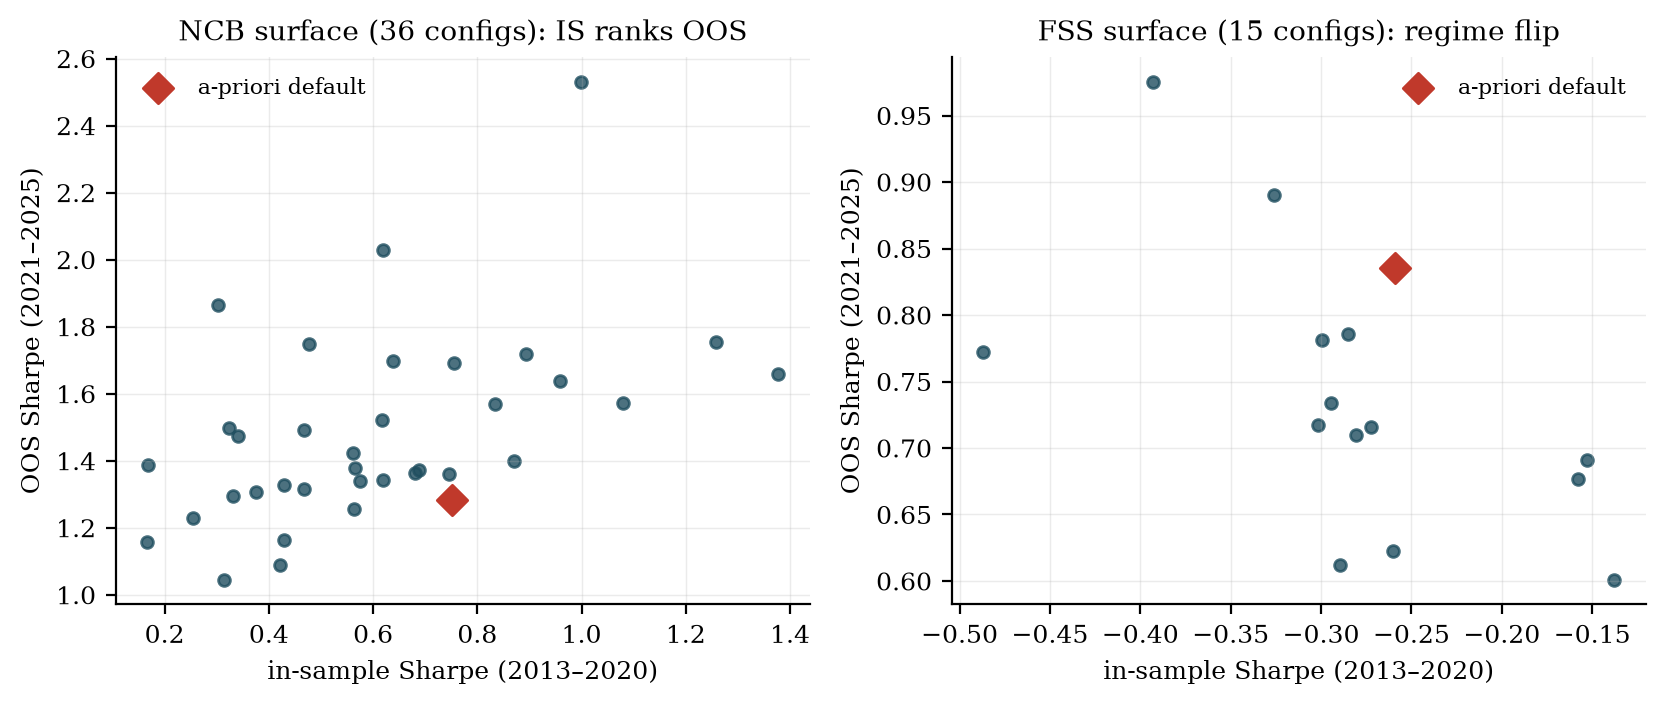
\includegraphics[width=.95\linewidth]{figs/f7_surfaces.png}
\caption{In-sample (2013--2020) versus out-of-sample (2021--2025)
Sharpe by configuration. Left: NCB, 36 configurations --- the whole
surface is OOS-positive and the in-sample ordering predicts the OOS
ordering (rank corr.\ $+0.53$); selection is meaningful, the default
(diamond) is conservative mid-surface. Right: FSS, 15 configurations
--- the surface moves as one block across a regime flip and the IS
ordering \emph{anti-predicts} OOS (rank corr.\ $-0.81$): the correct
use of the selection protocol is to refuse to select.}
\label{fig:surfaces}
\end{figure}

\begin{table}[h]
\centering\scriptsize
\caption{NCB surface, top rows and default (full 36-row table in the
repository). Coupled moving-block bootstrap (block 4, $B=2{,}000$);
selection statistic $=$ 5th percentile of bootstrap Sharpe.}
\begin{tabular}{lrrrrr}
\toprule
config (w-quantile / growth / min holders) & IS Sharpe & boot p05 &
OOS Sharpe & OOS $t$ \\
\midrule
0.95 / 1.50 / 3 (both selectors' pick) & $+1.38$ & $+0.92$ & $+1.66$ & $+4.85$ \\
0.95 / 1.50 / 5 & $+1.26$ & $+0.72$ & $+1.76$ & $+5.08$ \\
0.95 / 1.50 / 10 (best OOS) & $+1.00$ & $+0.49$ & $+2.53$ & $+5.44$ \\
\textbf{0.90 / 1.25 / 5 (a-priori default)} & $+0.75$ & $+0.14$ & $+1.28$ & $+3.31$ \\
worst on grid & $+0.17$ & $-0.34$ & $+1.39$ & $+3.93$ \\
\bottomrule
\end{tabular}
\end{table}

\begin{table}[h]
\centering\scriptsize
\caption{FSS surface (threshold $\times$ basket fraction),
index-hedged short-leg Sharpe. All fifteen configurations lose
modestly in-sample and pay out-of-sample: a regime, not a
hyperparameter.}
\begin{tabular}{lrrrr}
\toprule
config & IS Sharpe & boot p05 & OOS Sharpe & OOS $t$ \\
\midrule
$-$0.05 / top 10\% & $-0.14$ & $-0.57$ & $+0.60$ & $+1.87$ \\
\textbf{$-$0.10 / top 20\% (default)} & $-0.26$ & $-0.75$ & $+0.84$ & $+2.84$ \\
$-$0.20 / top 20\% (best OOS) & $-0.39$ & $-1.05$ & $+0.98$ & $+4.02$ \\
\bottomrule
\end{tabular}
\end{table}


\end{document}
